\documentclass[12pt, a4paper]{book}
\usepackage{geometry}
\geometry{a4paper, left=3cm, right=3cm, top=2cm, bottom=2cm} % Ajusta estos valores según necesites
\usepackage{lmodern}
\usepackage{amssymb,amsmath}
\usepackage{ifxetex,ifluatex}
\usepackage[spanish]{babel}
\usepackage{fixltx2e}
\usepackage{graphicx}
\usepackage{titlesec}

\titleformat{\chapter}[display]
  {\normalfont\Large\bfseries\centering}
  {\chaptername\ \thechapter}
  {20pt}
  {\Huge}
\titlespacing*{\chapter}{0pt}{-30pt}{20pt}

\ifnum 0\ifxetex 1\fi\ifluatex 1\fi=0
  \usepackage[T1]{fontenc}
  \usepackage[utf8]{inputenc}
\else
  \ifxetex
    \usepackage{mathspec}
  \else
    \usepackage{fontspec}
  \fi
  \defaultfontfeatures{Ligatures=TeX,Scale=MatchLowercase}
\fi
\usepackage[]{microtype}
\UseMicrotypeSet[protrusion]{basicmath}
\usepackage[unicode=true]{hyperref}
\hypersetup{
            pdfborder={0 0 0},
            breaklinks=true}
\urlstyle{same}
\usepackage{float}
\usepackage{parskip}
\setlength{\emergencystretch}{3em}
\providecommand{\tightlist}{%
  \setlength{\itemsep}{0pt}\setlength{\parskip}{0pt}}
\ifx\paragraph\undefined\else
\let\oldparagraph\paragraph
\renewcommand{\paragraph}[1]{\oldparagraph{#1}\mbox{}}
\fi
\ifx\subparagraph\undefined\else
\let\oldsubparagraph\subparagraph
\renewcommand{\subparagraph}[1]{\oldsubparagraph{#1}\mbox{}}
\fi
\makeatletter
\def\fps@figure{htbp}
\makeatother

\usepackage{fancyhdr}
\pagestyle{fancy}
\fancyhf{} % Limpia todos los encabezados y pies de página

% Configuración de encabezados
\fancyhead[LE]{\small\thepage} % Número de página a la izquierda (páginas pares)
\fancyhead[RO]{\small\thepage} % Número de página a la derecha (páginas impares)
\fancyhead[RE,LO]{\small\chaptername\ \thechapter. \leftmark} % "Capítulo X. Título"

% Línea divisoria
\renewcommand{\headrulewidth}{0.4pt} % Grosor de la línea
\renewcommand{\headrule}{\hrule width\headwidth height\headrulewidth \vskip-\headrulewidth}

% Formateo de los títulos de capítulos
\renewcommand{\chaptermark}[1]{\markboth{#1}{}} % Elimina "Capítulo X" del encabezado

% Estilo para páginas de inicio de capítulo (sin encabezado excepto número de página)
\fancypagestyle{plain}{%
  \fancyhf{}
  \fancyfoot[C]{\thepage}
  \renewcommand{\headrulewidth}{0pt}
}


% Comando para la portada
\newcommand{\portada}[5]{ % #1=Título, #2=Autor, #3=Tutor, #4=Título académico, #5=Fecha
  \begin{titlepage}
    \begin{center}
      % Parte superior
      {\normalsize FACULTAD DE MATEMÁTICA Y COMPUTACIÓN} \\
      {\normalsize UNIVERSIDAD DE LA HABANA} \\
      \vspace{1cm}
      
\includegraphics[width=0.3\textwidth]{images/uhlogo.png} \\
      \vspace{2cm}
      
      % Título
      {\LARGE \textbf{#1}} \\
      \vspace{2cm}
      
      % Autor y tutor
      \begin{tabular}{l l}
        \textbf{Autor:} & #2 \\
        \textbf{Tutor:} & #3 \\
      \end{tabular}
      \vspace{2cm}
      
      % Pie de portada
      \textbf{TRABAJO DE DIPLOMA} \\
      Presentado en opción al título de \\
      \textbf{#4} \\
      \vfill
      #5 % Fecha
    \end{center}
  \end{titlepage}
}



% En el preámbulo (antes de \begin{document})
\newenvironment{opiniontutor}
{
  \cleardoublepage
  \thispagestyle{empty}
  \begin{center}
    {\LARGE\bfseries OPINIÓN DEL TUTOR} \\[1.5cm] % Título grande
  \end{center}
  \setlength{\parskip}{1em} % Espacio entre párrafos
}
{
  \vspace{3cm} % Espacio para firma
  \begin{flushright}
    
\includegraphics[width=6cm]{images/firma_tutor.png} \\ % Ajusta el ancho y la ruta
    \vspace{0.5cm} % Espacio entre firma y texto
    \textbf{MSc. Joanna Campbell Amos} \\
    \textbf{Facultad de Matemática y Computación} \\
    \textbf{Universidad de La Habana}
  \end{flushright}
}

% En el preámbulo (antes de \begin{document})
\newenvironment{agradecimientos}{
  \clearpage % Usa \clearpage en lugar de \cleardoublepage
  \thispagestyle{empty} % Página sin número
  \begin{center}
    {\LARGE\bfseries AGRADECIMIENTOS} \\[1.5cm]
  \end{center}
  \setlength{\parindent}{0pt} % Sin sangría
  \setlength{\parskip}{1em} % Espacio entre párrafos
}{
  \vspace*{\fill} % Espacio flexible hasta el final
  \newpage % Opcional: si quieres asegurar nueva página después
}

% En el preámbulo (antes de \begin{document})
\newenvironment{resumentesis}[1]{ % #1 = título del trabajo
  \clearpage
  \thispagestyle{empty}
  \begin{center}
    {\LARGE\bfseries RESUMEN} \\[1.5cm]
  \end{center}
  \setlength{\parskip}{1em} % Espacio entre párrafos
}{
  \vspace{1cm}
  \noindent
  \textbf{Palabras clave:} \\[0.3cm]
  \hspace*{1.5cm} % Sangría para las palabras clave
  \begin{minipage}{0.8\textwidth}
    \textit{GeoBase, aplicación móvil, recopilación de datos, formulario, multimedia}
  \end{minipage}
  \newpage
}

% En el preámbulo (antes de \begin{document})
\newenvironment{abstractpage}[1]{ % #1 = título del trabajo en inglés
  \clearpage
  \thispagestyle{empty}
  \selectlanguage{english} % Cambia temporalmente a inglés
  \begin{center}
    {\LARGE\bfseries ABSTRACT} \\[1.5cm]
  \end{center}
  \setlength{\parskip}{1em} % Espacio entre párrafos
}{
  \vspace{1cm}
  \noindent
  \textbf{Keywords:} \\[0.3cm]
  \hspace*{1.5cm} % Sangría para las palabras clave
  \begin{minipage}{0.8\textwidth}
    \textit{GeoBase, mobile application, data collection, form, multimedia}
  \end{minipage}
  \selectlanguage{spanish} % Vuelve al español
  \newpage
}


\let\cleardoublepage\clearpage % Elimina páginas en blanco

\date{}

\begin{document}

\portada
  {Geobase 2.0: Soporte a formularios dinámicos anidados} % Título
  {Alfredo Nuño Oquendo}                % Autor
  {MSc. Joanna Campbell Amos}           % Tutor
  {Licenciado en Ciencias de la Computación} % Título académico
  {La Habana, \today}                       % Fecha

\begin{agradecimientos}
  Deseo expresar mi más sincero agradecimiento a:
  
  \begin{itemize}
    \item En primer lugar agradecer a Dios, todo lo que soy es gracias a su inmerecida misericordia y su gran amor.
    \item A mi tutora, MSc. Joanna Campbell Amos, por su guía constante, su infinita paciencia y preocupación.
    \item A todos los excelentes profesores de la facultad que a lo largo de estos 4 años me han instruido y me han hecho ver todo un mundo nuevo de conocimientos.
    \item A mi familia, que a pesar de estar lejos, siempre los he sentido muy cerca y presente, los amo demasiado.
    \item Tuve la dicha de compartir en mi año con personas muy talentosas no solo en el ámbito de las ciencias, las cuales siempre me impulsaron a mejorar. 
    \item Entre las bendiciones que Dios nos da a todos está poner en nuestro camino personas que no solo son amistades, sino que son como hermanos, personas que nos edifican espiritualmente. Estoy muy agradecido con Dios por haber compartido con el grupo cristiano universitario (GCU), son verdaderamente sal y luz en un contexto cada vez más complicado y hostil.
    \item Un agradecimiento especial a ``los calaveras'', juntos tiramos código de madrugada y minutos antes de la hora de entrega. Va por ustedes:
    \begin{figure}[H]
      \centering
      
\includegraphics[width=0.3\textwidth]{images/meme-calaveras.jpg}
      \label{fig:skull}
    \end{figure} 
    \item No podía faltar el GCU de Bahía, tanto los que se fueron como los que están en este momento, aprendí y me divertí mucho con ustedes, sobre todo en los tiempo de ciclón y apagón general, convierten esos momentos terribles en tiempos que me gustaría volver a vivir junto a ellos (Rosalia, Kevin, Felipe, Héctor, Jonathan, Yandris, Magniel, Aser, Thalia, Lia, Liannis, Susanna, Daniel, Armin, Roxana, Neidys, Yaneyra, Jorgito, Dayron, Yan Carlos, William). En especial me siento muy agradecido por haber conocido a dos personitas: Dayanis, una prestigiosa meteoróloga tunera que no le gusta coger sol, y a una guantanamera que no se le acaban las pilas, nos conocimos en un ciclón y desde entonces hemos pasado muchos ciclones juntos, y espero pasar muchos más contigo.
  \end{itemize}
  
  \end{agradecimientos}

\begin{opiniontutor}
  El trabajo presentado como tesis de culminación de estudios de licenciatura por la estudiante Alfredo Nuño Oquendo  constituye un ejemplo de la aplicación de conocimientos y habilidades adquiridas durante sus años de estudio, combinados con la utilización de su capacidad de investigación para la generación de ideas, asimilación de tecnologías y creación de soluciones al problema planteado.

  Para cumplir con los objetivos propuestos, realizó una ardua labor investigativa en temas totalmente nuevos para él, relacionados con las tecnologías presentes en los dispositivos móviles actuales y con la amplia temática de los Sistemas de Información Geográfica.

  Este esfuerzo se materializa en lo expuesto en los Capítulos 1 y 2, donde recoge el estado del arte relacionado con los objetivos de este trabajo de diploma, tanto desde el punto de vista teórico-conceptual como tecnológico y en el Capítulo 3, propone e implementa  una solución teórico- computacional  para solucionar su problemática haciendo uso de la tecnología asimilada. Independencia, dedicación, perseverancia, profesionalidad, capacidad e iniciativa son algunos de los calificativos que merece la labor de Alfredo.

  El trabajo que Alfredo presenta hoy en su ejercicio de fin de carrera es el resultado de un año  de arduo trabajo, que contra todo pronóstico, adversidades se pudo llevar a término.  Como tutora estoy satisfecha con el trabajo desarrollado aunque quedaron cosas por hacer  y mejorar. Considero que desde el punto de vista académico, satisface los requerimientos de una tesis de licenciatura y cumple con los objetivos que nos trazamos para la misma al inicio de esta etapa.

  Por todo lo anterior propongo al tribunal que se le otorgue la calificación de Excelente (5).

\end{opiniontutor}

% Después de portada y antes de índices
\begin{resumentesis}
  
  GeoBase es una aplicación móvil cartográfica desarrollada por la Casa del Software de la Facultad de Matemática y Computación de la Universidad de La Habana, que permite recopilar información asociada a ubicaciones específicas mediante formularios dinámicos configurados por el usuario. En este trabajo se presenta una mejora a GeoBase con la incorporación de nuevas funcionalidades en su capacidad de recolección de datos en campo. Se destacan la incorporación de formularios anidados, que permiten una captura de información más detallada y estructurada, la incorporación de archivos multimedia, y la adaptación de la aplicación para facilitar la recopilación de datos que tributen directamente a la resolución de problemas de optimización, como el diseño de recorridos eficientes. 

  Mediante el caso de uso que consiste en la recopilación de datos en campo de la empresa eléctrica, se evidenció la utilidad de esta nueva versión de GeoBase ya que se hizo necesario el empleo de los formularios anidados (organizados en categorías como “Postes eléctricos” y subcategorías como “Transformadores”, entre otras) y datos multimedia (fotos, videos, notas de voz) para documentar daños. La aplicación georreferencia cada punto y exporta la información que será utilizada en un algoritmo de optimización de rutas, lo cual permitirá priorizar reparaciones urgentes y minimizar tiempos y costos. Esto mejorará la eficiencia del mantenimiento y el suministro eléctrico en las comunidades.

\end{resumentesis}


\begin{abstractpage}
  
  GeoBase is a mobile cartographic application developed by the Software House of the Faculty of Mathematics and Computer Science at the University of Havana. It allows the collection of information associated with specific locations through user-configured dynamic forms. This work presents an enhancement to GeoBase by incorporating new functionalities to improve its field data collection capabilities. Notable improvements include the addition of nested forms, which enable more detailed and structured information capture, the integration of multimedia files, and the adaptation of the application to facilitate data collection that directly contributes to solving optimization problems, such as designing efficient routes.

  Through the use case involving field data collection for an electric company, the usefulness of this new version of GeoBase was demonstrated. The need arose to employ nested forms (organized into categories such as “Electric Poles” and subcategories like “Transformers,” among others) and multimedia data (photos, videos, voice notes) to document damages. The application georeferences each point and exports the information to be used in a route optimization algorithm, which will allow prioritizing urgent repairs and minimizing time and costs. This will enhance the efficiency of maintenance and electrical supply in the communities.

  \end{abstractpage}

% Tabla de contenido (índice)
\tableofcontents

% Lista de figuras (opcional)
\listoffigures

\chapter{Introducción}

El manejo de la información geográfica es una disciplina fundamental en la actualidad, dada su relevancia para la localización, el análisis espacial y la toma de decisiones en diversos ámbitos. Los Sistemas de Información Geográfica (SIG o GIS por sus siglas en inglés \cite{sarria2020}) han evolucionado significativamente, integrando datos espaciales con información socioeconómica y ambiental, lo que ha permitido abordar problemas complejos con mayor precisión y eficacia. Esta evolución ha sido impulsada por el desarrollo tecnológico, especialmente con la expansión de las aplicaciones móviles, que han facilitado la captura y gestión de datos georreferenciados directamente en el campo.

Las aplicaciones móviles basadas en mapas se han convertido en herramientas esenciales para el levantamiento de información en terreno, permitiendo a los usuarios recopilar datos asociados a ubicaciones específicas mediante formularios dinámicos y configurables. Estas herramientas ofrecen portabilidad, facilidad de uso y seguridad en el almacenamiento y transporte de la información desde zonas remotas hasta los centros de procesamiento y análisis. La integración de sensores y capacidades multimedia en los dispositivos móviles ha ampliado las posibilidades de documentación y enriquecimiento de los datos recolectados.

En este contexto, la evolución de los SIG ha estado marcada por la transición desde sistemas estáticos y centralizados hacia plataformas móviles y dinámicas que permiten la interacción en tiempo real con la información geográfica. Esta transformación ha abierto nuevas oportunidades para mejorar la eficiencia y calidad del levantamiento de datos en campo, así como para facilitar su análisis y aplicación en la resolución de problemáticas territoriales, sociales y ambientales. La presente investigación se enmarca en esta línea de desarrollo, enfocándose en la mejora de una aplicación móvil cartográfica para optimizar la captura y gestión de datos georreferenciados mediante formularios anidados \cite{ceri1984}, validación dinámica y soporte multimedia.

\section{Antecedentes del problema
científico}\label{antecedentes-del-problema-cientuxedfico}
La Casa del Software de la Facultad de Matemática y Computación de la Universidad de La Habana desarrolló diversas soluciones en el ámbito de los Sistemas de Información Geográfica (SIG), destacándose proyectos como OpenLatino GIS y varias tesis orientadas a aplicaciones móviles para la captura y gestión de datos espaciales. Entre estas investigaciones previas se encuentra la tesis ``Aplicaciones móviles  para la recogida y notificación de datos en campo sobre las propiedades de Managua, Nicaragua'' de Sheyla Cruz Castro \cite{castro2018}, que propuso dos aplicaciones móviles (Encuestador y Notificador). Estas aplicaciones permiten registrar información asociada a propiedades utilizando formularios sobre una cartografía offline, con datos iniciales proporcionados por un servicio externo. Aunque ofrecen funcionalidades básicas de captura y notificación, su estructura de formularios es estática y carecen de flexibilidad para adaptarse a diferentes escenarios o necesidades de levantamiento en campo, además de que el soporte multimedia se limita a imágenes. También encontramos la tesis ``NTCollector: aplicación móvil para manejo de redes geográficas con formularios dinámicos'' de Abraham González Rivero \cite{rivero2019}, la cual presentó la aplicación NTCollector, diseñada para el manejo de redes geográficas y la recolección de datos mediante formularios dinámicos en campo. NTCollector permite la configuración de formularios y la visualización de datos sobre mapas, pero su modelo de persistencia se basa en archivos JSON y no en una base de datos robusta, lo que limita la escalabilidad y gestión eficiente de grandes volúmenes de datos. Además, la aplicación no contempla el manejo avanzado de multimedia, y su integración con mapas offline y online depende de configuraciones externas.

GeoBase, en su versión inicial, fue diseñada para permitir la captura de información georreferenciada mediante formularios dinámicos configurados a través de la definición de categorías. Cada punto de interés, que incluye un componente geoespacial, se asocia a una categoría específica con su correspondiente formulario personalizado, facilitando así la recolección adaptable de datos según las necesidades del usuario. La aplicación implementa una arquitectura multicapa basada en Clean Architecture, que garantiza la extensibilidad en varios aspectos clave: permite integrar diversas fuentes cartográficas, principalmente mediante servicios WMS; soporta la definición flexible de tipos de columnas y formatos de datos en los formularios; y es extensible en cuanto a los tipos de medios que se pueden asociar a los datos. En cuanto a la persistencia, GeoBase utiliza una base de datos local SQLite, con un diseño abierto que posibilita la incorporación de otros mecanismos de almacenamiento en el futuro.

A pesar de las ventajas que ofrece la versión inicial de GeoBase, esta presenta varias limitaciones que motivan su evolución. Entre ellas se encuentra la falta de soporte para el manejo de tipos de medios como video, QR y audio, lo que restringe la capacidad de enriquecer la información recolectada en campo. Además, no cuenta con mecanismos integrados para exportar los puntos guardados a diferentes formatos, limitando la interoperabilidad y el análisis externo de los datos. La aplicación tampoco permite recibir un conjunto de puntos, mostrarlos en el mapa y completar su información, lo cual retrasa el proceso de llenado de datos cuando ya se sabe toda la información geográfica de los puntos. Otro aspecto pendiente es la serialización de los metadatos de las categorías con sus columnas, necesaria para cargar configuraciones de formularios de manera eficiente, optimizando el proceso de crear categorías que ya existen en otros dispositivos. Asimismo, GeoBase no implementa formularios anidados, lo que limita la captura de información jerárquica o dependiente, ni dispone de mecanismos de búsqueda para facilitar la localización rápida de datos dentro de la aplicación. Finalmente, la versión inicial carece de validación dinámica de campos en los formularios, es decir, no permite que el usuario defina reglas o restricciones específicas para cada campo, lo que podría mejorar la calidad y coherencia de los datos recolectados. Estas carencias evidencian la necesidad de desarrollar nuevas funcionalidades que amplíen la flexibilidad, usabilidad y capacidad de gestión de GeoBase para responder mejor a las demandas actuales del trabajo de campo y la gestión eficiente de la información espacial.

\section{Presentación de la
problemática}\label{presentaciuxf3n-de-la-problemuxe1tica}

El problema central que aborda este trabajo es la necesidad de extender las funcionalidades de GeoBase para soportar formularios anidados y estructuras complejas, que permitan una captura más detallada y organizada de la información. También, se requiere implementar exportación de la información recolectada a distintos formatos (Excel, JSON, etc), lo que facilita su integración con otros sistemas y herramientas de análisis, y de las categorías no solo exportar su información en formato JSON, sino también cargarla, para optimizar el trabajo. La inclusión de soporte para nuevos tipos de campos en los formularios, como video, audio y QR es también una necesidad para documentar con mayor riqueza los puntos de interés. Estas mejoras son especialmente relevantes en contextos como la gestión de infraestructuras eléctricas en zonas rurales, donde la precisión y rapidez en la recolección y análisis de datos impactan directamente en la eficiencia del mantenimiento y la calidad del servicio.

En este contexto, el objeto de estudio de este trabajo es la aplicación móvil GeoBase y su base de datos para la gestión de formularios dinámicos y datos georreferenciados.

El campo de acción abarca las aplicaciones móviles para la recolección y gestión de datos georreferenciados, con énfasis en la optimización de procesos y toma de decisiones en sectores como la gestión de infraestructuras.

En este punto es válido preguntarnos: ¿Cómo desarrollar una aplicación móvil capaz de manejar datos georreferenciados mediante formularios dinámicos y anidados, que incluya soporte para tipos de medios como video, QR y audio, y que además facilite la recolección, visualización y análisis de información en campo? ¿Cómo implementar mecanismos eficientes para la exportación de datos en múltiples formatos y la serialización y carga de configuraciones de categorías y formularios?

\section{Motivación y
justificación}\label{motivaciuxf3n-y-justificaciuxf3n}

La integración de tecnologías móviles y SIG es una tendencia clave para la gestión eficiente de datos geoespaciales. La capacidad de generar formularios dinámicos y anidados, junto con la incorporación de medios multimedia permite obtener una información más completa y confiable. Esta información, a su vez, puede ser utilizada en algoritmos de optimización para resolver problemas prácticos como la planificación de rutas eficientes, priorización de tareas y reducción de costos operativos.

La mejora de GeoBase se enmarca en este contexto, buscando ofrecer una herramienta flexible y robusta que responda a las demandas actuales del trabajo de campo en diversos sectores. En el ámbito práctico, la implementación de nuevas funcionalidades a GeoBase mejora la captura y análisis de datos en campo, impactando positivamente en sectores como la gestión eléctrica rural, donde la priorización de reparaciones y la optimización de rutas pueden traducirse en ahorros significativos y mejor servicio a la comunidad.

Desde el punto de vista personal, cuento con la formación y los conocimientos necesarios para abordar este proyecto, adquiridos a lo largo de la carrera y mediante el análisis de aplicaciones previas que sirven de base para el desarrollo de las nuevas funcionalidades de GeoBase. Además, la participación en foros de Flutter y la asesoría directa del desarrollador original de GeoBase me han permitido profundizar en las mejores prácticas y soluciones técnicas, asegurando la viabilidad y calidad de la implementación propuesta.

\section{Objetivos}\label{objetivos}

El objetivo general de este trabajo es extender las funcionalidades de GeoBase para soportar formularios dinámicos anidados, exportar y cargar configuraciones de categorías en formato JSON, incluir soporte para tipos de medios de video, audio y QR e implementar exportación de los datos recolectados a formato Excel.

\textbf{Objetivos específicos:}
\begin{itemize}
    \item Extender la base de datos para soportar formularios dinámicos con múltiples instancias anidadas y estructuras jerárquicas.
    \item Implementar un mecanismo eficiente para la exportación de la información recolectada, incluyendo la generación de archivos en formato Excel.
    \item Ampliar el soporte multimedia en los formularios, integrando video, audio, imágenes y códigos QR.
    \item Mejorar la interfaz de usuario mediante widgets especializados que faciliten la creación y eliminación de formularios complejos en tiempo de ejecución.
    \item Documentar detalladamente el proceso de desarrollo e integración de las nuevas funcionalidades, y evaluar su impacto en la eficiencia y usabilidad del flujo de trabajo en campo.
\end{itemize}


\textbf{Objetivos parciales}
\begin{itemize}
    \item Contribuir al fortalecimiento de las capacidades de recolección y gestión de datos georreferenciados en aplicaciones móviles.
    \item Impulsar la interoperabilidad y el intercambio eficiente de datos entre diferentes plataformas y herramientas de análisis.
    \item Fomentar la mejora continua de la experiencia de usuario en aplicaciones de levantamiento de datos geográficos.
    \item Apoyar la toma de decisiones basada en información georreferenciada precisa y enriquecida con medios multimedia.
\end{itemize}

\section{Estructuración del
trabajo}\label{estructuraciuxf3n-del-trabajo}

La tesis se organiza en seis capítulos principales:

\begin{enumerate}
\def\labelenumi{\arabic{enumi}.}
\tightlist
\item
  \textbf{Introducción:} Presenta el contexto, antecedentes,
  problemática, motivación, justificación y objetivos del trabajo.
\item
  \textbf{Estado del arte:} Revisión de la literatura y tecnologías
  relacionadas con los SIG móviles, la recolección de datos
  georreferenciados y el uso de formularios anidados.
\item
  \textbf{Diseño e implementación de la propuesta de solución:} Describe el estado inicial de GeoBase, los cambios realizados, los métodos más relevantes y los paquetes utilizados, además de algunos detalles de implementación y estructura.
\item
  \textbf{Caso de estudio:} Presenta la validación de resultados mediante la aplicación de la solución en un escenario real, incluyendo documentación fotográfica de la aplicación en uso.
\item
  \textbf{Conclusiones y recomendaciones:} Resume los principales
  hallazgos, limitaciones y posibles líneas futuras de trabajo.
\item
  \textbf{Bibliografía} Incluye la bibliografía utilizada.
\end{enumerate}















\chapter{Estado del arte}\label{estadodelarte}

En este capítulo, tras una revisión exhaustiva del panorama actual, se analizan algunas de las aplicaciones móviles que hoy en día ofrecen funcionalidades similares a las que se propone incorporar en la aplicación objeto de esta tesis. Este análisis permite identificar tanto las capacidades existentes en el sector de las aplicaciones SIG móviles como las limitaciones que presentan respecto a los nuevos requerimientos planteados.

\section{Aplicaciones con funcionalidades similares}

\subsection{ArcGIS Field Maps}

ArcGIS Field Maps \cite{esriFieldMaps} es una aplicación móvil todo en uno desarrollada por Esri que permite a los usuarios recopilar datos en campo, visualizar mapas y compartir ubicaciones en tiempo real desde un único entorno integrado. Está disponible para dispositivos Android, iOS y watchOS, y se integra plenamente con la plataforma ArcGIS Online, facilitando la sincronización de datos y la gestión centralizada.

\begin{figure}[h]
  \centering
  
\includegraphics[width=0.4\textwidth]{images/arcgis_logo.png}
  \caption{Logo de ArcGIS Field Maps}
  \label{fig:arcgisfieldmapslogo}
\end{figure}

\textbf{Funcionamiento general:}
\begin{itemize}
  \item \textbf{Captura y edición de datos geográficos:} Permite a los usuarios capturar y actualizar puntos, líneas y polígonos, así como editar atributos asociados directamente sobre mapas configurados en ArcGIS. Los usuarios pueden trabajar con capas habilitadas para edición y aplicar plantillas de entidades para estandarizar la recolección de datos.
  
  \item \textbf{Formularios inteligentes:} Ofrece formularios configurables basados en mapas, con capacidad para agrupar atributos, definir orden y aplicar lógica condicional para mostrar u ocultar campos, mejorando la experiencia de recolección. Los formularios pueden incluir campos obligatorios, valores predeterminados y listas desplegables dinámicas.
  
  \item \textbf{Soporte multimedia:} Los usuarios pueden adjuntar fotos, videos y audios a las entidades geográficas, enriqueciendo la información recolectada. Los archivos multimedia se almacenan como parte de los atributos de la entidad y pueden visualizarse tanto en campo como en oficina.
  
  \item \textbf{Trabajo offline:} Permite descargar mapas para trabajar sin conexión, sincronizando los datos cuando se restablece la conectividad. Los mapas offline incluyen tiles basados en vectores para un rendimiento optimizado y bajo consumo de almacenamiento.
  
  \item \textbf{Ubicación en tiempo real:} Registra y comparte la ubicación del usuario, incluso en segundo plano, integrando datos de sensores del dispositivo para mejorar la precisión y el contexto de la actividad. Soporta el seguimiento continuo de flotas o equipos de campo.
  
  \item \textbf{Integración con otras apps Esri:} Facilita la simplificación de flujos de trabajo al integrarse con aplicaciones como ArcGIS Workforce para la gestión de tareas y ArcGIS Navigator para la navegación guiada.
\end{itemize}

\begin{figure}[h]
  \centering
  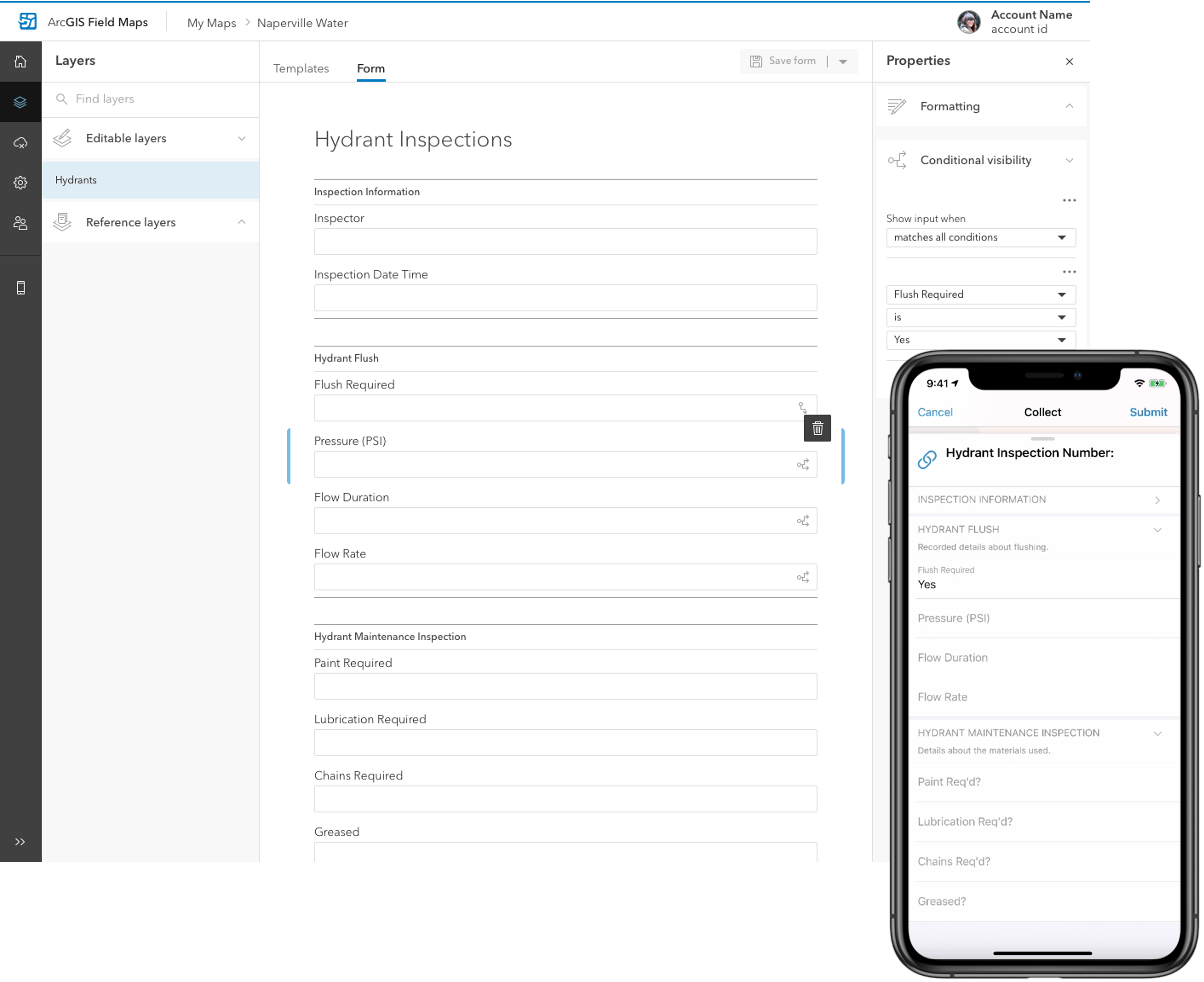
\includegraphics[width=0.5\textwidth]{images/FieldMapsSmartForms.png}
  \caption{Formulario inteligente en ArcGIS Field Maps}
  \label{fig:fieldmapsform}
\end{figure}

\textbf{Limitaciones:}
\begin{itemize}
  \item \textbf{Formularios anidados complejos:} Aunque permite agrupar atributos y usar lógica condicional, no soporta formularios anidados con estructuras jerárquicas profundas ni formularios recursivos como los que se plantean para GeoBase. Esto limita la captura de datos con múltiples niveles de relaciones padre-hijo.
  
  \item \textbf{Carga y exportación/importación de configuraciones:} No ofrece funcionalidades nativas para cargar o exportar configuraciones de categorías o formularios en formatos estándar como JSON, lo que limita la portabilidad y reutilización de configuraciones avanzadas entre proyectos o organizaciones.
  
  \item \textbf{Soporte multimedia extendido:} Aunque permite fotos y videos, no integra otros tipos de medios como códigos QR ni ofrece un manejo multimedia tan flexible dentro de formularios dinámicos anidados. Tampoco permite la edición básica de imágenes directamente en la aplicación.
  
  \item \textbf{Independencia tecnológica:} Está fuertemente vinculado al ecosistema Esri y requiere licencias específicas, lo que puede limitar su adopción en entornos que buscan soluciones más abiertas o personalizables. La integración con sistemas externos no basados en ArcGIS es compleja.
\end{itemize}

\subsection{Mergin Maps}

Mergin Maps \cite{merginmapsdocs} es una aplicación móvil de código abierto diseñada para la recolección y edición de datos geoespaciales en campo, con una integración nativa y fluida con QGIS \cite{qgisdocs}, uno de los sistemas de información geográfica (SIG) más utilizados en el mundo. Su interfaz intuitiva y simplificada permite que usuarios con poca experiencia en SIG puedan comenzar a recopilar y editar datos rápidamente, facilitando la adopción en equipos diversos.

\begin{figure}[h]
  \centering
  
\includegraphics[width=0.5\textwidth]{images/mergin_maps.jpeg}
  \caption{Logo de Mergin Maps}
  \label{fig:merginlogo}
\end{figure}

\textbf{Funcionamiento general:}
\begin{itemize}
  \item \textbf{Captura y edición de datos geoespaciales:} Permite agregar y modificar puntos, líneas y polígonos directamente sobre mapas, con formularios personalizados configurados desde QGIS. Los usuarios pueden editar tanto geometrías como atributos con gestos táctiles intuitivos.
  
  \item \textbf{Interfaz amigable:} No utiliza modos separados para explorar o editar; los usuarios pueden tocar cualquier elemento en el mapa para ver detalles y editar atributos o geometría con facilidad. La interfaz se adapta automáticamente entre modo horizontal y vertical.
  
  \item \textbf{Formularios personalizados:} Los formularios se diseñan en QGIS, permitiendo la inclusión de campos con etiquetas claras y opciones configurables para la recolección de datos. Soporta campos de texto, numéricos, fechas, listas desplegables y casillas de verificación.
  
  \item \textbf{Soporte multimedia:} Integra captura de fotos, videos y grabaciones de audio vinculadas a los datos geográficos, enriqueciendo la información recolectada. Las fotos pueden georreferenciarse automáticamente con las coordenadas del dispositivo.
  
  \item \textbf{Trabajo offline y sincronización:} Funciona sin conexión, sincronizando los cambios con la nube mediante el servicio Mergin cuando hay conectividad disponible. Utiliza una tecnología eficiente de diferencias (Geodiff) para la sincronización y manejo de conflictos, minimizando el uso de datos.
  
  \item \textbf{Control de versiones y gestión multiusuario:} Permite que múltiples usuarios editen simultáneamente un proyecto, con control de versiones y resolución de conflictos. Mantiene un historial completo de cambios con autoría y timestamps.
  
  \item \textbf{Compatibilidad con receptores GNSS externos:} Mejora la precisión de la captura de datos geográficos al conectarse con dispositivos GPS profesionales vía Bluetooth o cable.
  
  \item \textbf{Interoperabilidad con QGIS:} La sincronización facilita la transferencia directa de datos entre campo y escritorio, optimizando los flujos de trabajo SIG. Los proyectos creados en QGIS con plugins específicos pueden desplegarse directamente en la app móvil.
\end{itemize}

\begin{figure}[h]
  \centering
  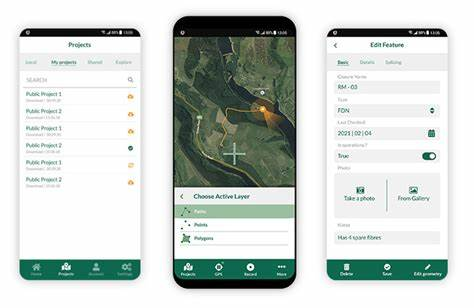
\includegraphics[width=0.5\textwidth]{images/mergin.jpeg}
  \caption{Interfaz de usuario de Mergin Maps}
  \label{fig:merginform}
\end{figure}

\textbf{Limitaciones:}
\begin{itemize}
  \item \textbf{Formularios anidados complejos:} Aunque permite formularios personalizados, no soporta formularios anidados con estructuras jerárquicas profundas ni lógica recursiva, limitando la captura de datos con múltiples niveles de dependencia. Las relaciones entre tablas deben gestionarse manualmente.
  
  \item \textbf{Gestión de configuraciones:} La carga y exportación/importación de configuraciones de categorías y formularios no se realiza directamente desde la app ni en formatos estándar como JSON, sino que depende de la configuración previa en QGIS, lo que reduce la flexibilidad y portabilidad entre proyectos.
  
  \item \textbf{Manejo multimedia avanzado:} Aunque soporta fotos, videos y audio, no integra otros tipos de medios como códigos QR ni ofrece un manejo multimedia tan flexible dentro de formularios anidados como se propone en GeoBase. La visualización de medios en el mapa es limitada.
  
  \item \textbf{Dependencia de QGIS para configuración:} Requiere conocimientos técnicos y manejo de QGIS para diseñar y ajustar formularios y proyectos, lo que puede ser una barrera para usuarios sin experiencia en SIG. La curva de aprendizaje para configuraciones avanzadas es pronunciada.
\end{itemize}

\subsection{GIS Cloud Mobile Data Collection}

GIS Cloud Mobile Data Collection \cite{giscloudhow} es una aplicación móvil disponible para Android e iOS que permite la captura y actualización de datos georreferenciados en campo, con la capacidad de trabajar tanto en línea como offline. La plataforma GIS Cloud, de la cual forma parte esta app, fue lanzada en 2010, siendo pionera en soluciones GIS basadas en la nube.

\begin{figure}[h]
  \centering
  
\includegraphics[width=0.4\textwidth]{images/gis_cloud.png}
  \caption{Interfaz de usuario de Mergin Maps}
  \label{fig:giscloud}
\end{figure}

\textbf{Funcionalidades principales}

\begin{itemize}
\item \textbf{Formularios personalizados:} A través de un editor web intuitivo (Mobile Data Collection Portal), se pueden crear formularios ilimitados con múltiples tipos de campos, incluyendo texto, listas desplegables, botones de opción, casillas de verificación, firmas electrónicas, autocompletado, códigos de barras y QR, fotos y grabaciones de audio. Los formularios permiten campos obligatorios, condicionales (dependientes de otros campos) y persistentes para asegurar la calidad y coherencia de los datos.

\item \textbf{Captura geográfica:} Permite recolectar puntos, líneas y polígonos utilizando GPS o herramientas manuales de dibujo para mejorar la precisión en la ubicación.

\item \textbf{Trabajo offline:} La app funciona sin conexión, almacenando localmente los datos y sincronizándolos automáticamente cuando se restablece la conexión a internet.

\item \textbf{Visualización y edición en campo:} Los usuarios pueden revisar y editar atributos y medios adjuntos directamente desde la aplicación, así como escuchar grabaciones de audio y visualizar imágenes asociadas.

\item \textbf{Gestión de equipos y permisos:} Es posible asignar proyectos y formularios personalizados a diferentes usuarios, controlando permisos de recolección y actualización para optimizar la colaboración.

\item \textbf{Integración con plataforma GIS Cloud:} Los datos se sincronizan con la plataforma en la nube, donde se pueden gestionar, analizar y compartir mediante herramientas de edición de mapas, simbología avanzada, consultas espaciales, análisis y publicación de mapas.

\item \textbf{Funcionalidades adicionales:} Ubicación GPS en tiempo real, exploración de mapas en campo, interfaz renovada y soporte para inicio de sesión con múltiples proveedores (Google, Facebook, Salesforce, etc.).
\end{itemize}

\begin{figure}[h]
  \centering
  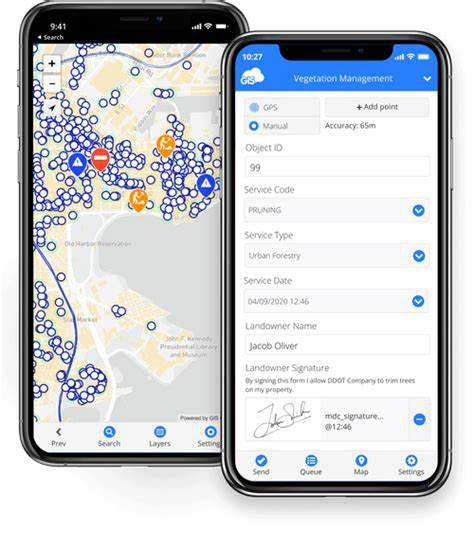
\includegraphics[width=0.4\textwidth]{images/gis_cloud_forms.jpeg}
  \caption{Interfaz de usuario de Mergin Maps}
  \label{fig:giscloudform}
\end{figure}

\textbf{Desventajas y limitaciones frente a las nuevas funcionalidades de GeoBase}

\begin{itemize}
\item \textbf{Formularios anidados complejos:} Aunque GIS Cloud Mobile Data Collection soporta formularios con campos condicionales y dependientes, no ofrece soporte para formularios anidados con estructuras jerárquicas profundas o recursivas como las que se proponen en GeoBase.

\item \textbf{Carga y exportación/importación de configuraciones:} No dispone de mecanismos nativos para cargar o exportar configuraciones completas de categorías o formularios en formatos estándar como JSON, lo que limita la portabilidad y reutilización avanzada de configuraciones.

\item \textbf{Mecanismos avanzados de búsqueda y actualización:} La app ofrece funcionalidades básicas de revisión y edición, pero carece de herramientas avanzadas para búsqueda eficiente, actualización masiva o gestión dinámica de grandes volúmenes de datos georreferenciados.

\item \textbf{Dependencia de plataforma en la nube:} El funcionamiento óptimo y la gestión de datos dependen de la plataforma GIS Cloud, lo que puede limitar la independencia tecnológica y la personalización en entornos con restricciones de conectividad o políticas de datos.
\end{itemize}

\section{Conclusiones de las aplicaciones presentadas}

A partir del análisis del estado del arte en aplicaciones móviles para la recolección de datos geoespaciales en campo, se observa que las soluciones actuales, como GIS Cloud Mobile Data Collection, ArcGIS Field Maps y Mergin Maps, han avanzado significativamente en la digitalización de procesos tradicionales. Estas aplicaciones permiten la captura de datos mediante formularios personalizados, integran soporte multimedia como fotos, audio y video, y ofrecen funcionalidades para trabajar en modo offline con sincronización en tiempo real. Esto ha contribuido a optimizar el flujo de trabajo, reducir errores y agilizar la gestión de información en entornos de campo.

No obstante, estas aplicaciones presentan limitaciones importantes en cuanto a la complejidad y flexibilidad de los formularios. La mayoría no soporta formularios anidados con estructuras jerárquicas profundas ni lógica recursiva, lo que restringe la capacidad para capturar datos en escenarios que requieren múltiples niveles de dependencia o categorización avanzada. Además, la gestión y portabilidad de configuraciones de formularios y categorías suele ser limitada, ya que no se ofrecen mecanismos nativos para cargar, exportar o importar configuraciones en formatos estándar como JSON, dificultando la reutilización y adaptación de formularios complejos entre distintos proyectos o equipos de trabajo. En relación con el manejo multimedia, aunque la mayoría de las aplicaciones soporta fotos, videos y grabaciones de audio, el soporte para otros tipos de medios, como códigos QR integrados en formularios, y la flexibilidad para su uso dentro de formularios dinámicos aún es incipiente. Finalmente, es importante destacar que muchas de estas aplicaciones están estrechamente vinculadas a ecosistemas tecnológicos específicos, como Esri, QGIS o GIS Cloud. Esta dependencia implica la necesidad de licencias, plataformas y conocimientos técnicos particulares, lo que puede afectar la flexibilidad, autonomía y accesibilidad para diversos usuarios y organizaciones.

En este contexto, resulta evidente que la incorporación de nuevas funcionalidades avanzadas en GeoBase, como formularios dinámicos y anidados, gestión flexible de configuraciones y multimedia, y mecanismos robustos de búsqueda y actualización, plantea desafíos significativos si se intentara integrar estas capacidades mediante el uso de APIs, librerías o aplicaciones existentes. Por estas razones, se justifica la decisión de implementar las funcionalidades en GeoBase desde cero, ya que este enfoque permite diseñar una arquitectura tecnológica abierta, modular y completamente adaptada a los requerimientos del proyecto, evitando las limitaciones y dependencias impuestas por soluciones preexistentes. Desarrollar la aplicación desde sus cimientos facilita la integración nativa de las funcionalidades deseadas, optimiza los recursos y garantiza mayor flexibilidad y autonomía tecnológica a largo plazo.

No obstante, es importante señalar que el análisis de las aplicaciones líderes en el sector ha sido fundamental para identificar buenas prácticas en el diseño de la interfaz de usuario y en la definición de flujos de interacción eficientes entre la aplicación y el usuario. Estas aplicaciones han servido como referencia y patrón para lograr una experiencia de usuario intuitiva y coherente, asegurando que GeoBase no solo innove en funcionalidad, sino también en usabilidad y eficiencia operativa en campo.










\chapter{Diseño e implementación de la propuesta de solución}

En este apartado se describen las decisiones tomadas en cuanto a la organización del modelo de datos, la arquitectura adoptada y las principales estrategias empleadas para extender las capacidades del sistema. El objetivo es detallar cómo se abordaron los desafíos técnicos derivados de la necesidad de gestionar estructuras de datos más complejas, como los formularios anidados, y cómo estas soluciones se integraron de manera coherente con la infraestructura existente, manteniendo la escalabilidad y mantenibilidad del sistema.

\section{Modelo de datos}

El modelo de datos implementado en GeoBase se compone de varias clases que permiten organizar y gestionar la información georreferenciada de manera estructurada y flexible. La clase \textbf{Geodata} representa los registros geográficos, almacenando las coordenadas espaciales y vinculándose con \textbf{Category}, que clasifica cada registro mediante atributos como nombre, color e icono. Por otro lado, la clase \textbf{Column} define los diferentes atributos o campos que pueden asociarse a cada categoría, y está relacionada tanto con \textbf{Category} como con \textbf{FieldType}, esta última encargada de especificar el tipo de dato y la forma en que debe ser interpretado o presentado.

Para manejar atributos especializados, el modelo incluye las clases \textbf{StaticSelection} y \textbf{Media}, las cuales se asocian con \textbf{FieldType} para definir opciones preestablecidas y tipos de archivos multimedia permitidos, respectivamente. Finalmente, la clase \textbf{FieldValue} almacena los valores concretos capturados, estableciendo una relación directa con \textbf{Geodata} y \textbf{Column}, lo que asegura que cada dato registrado esté correctamente asociado a su ubicación geográfica y a su atributo correspondiente. La Figura \ref{fig:oldmerx} representa el modelo anteriormente descrito, para más detalles consultar \cite{garcia2024}.

Aunque el modelo de datos descrito permite representar tipos de datos como códigos QR y videos (tratando el primero como un valor de tipo cadena y el segundo como un objeto multimedia asociado a \textbf{Media}), presenta limitaciones importantes para abordar la complejidad que implican los formularios anidados. Esto se debe a que la estructura actual está diseñada para almacenar valores individuales asociados a atributos planos mediante \textbf{FieldValue}, sin contemplar la posibilidad de que un campo pueda contener a su vez un conjunto de subcampos relacionados jerárquicamente.

\begin{figure}[H]
\centering
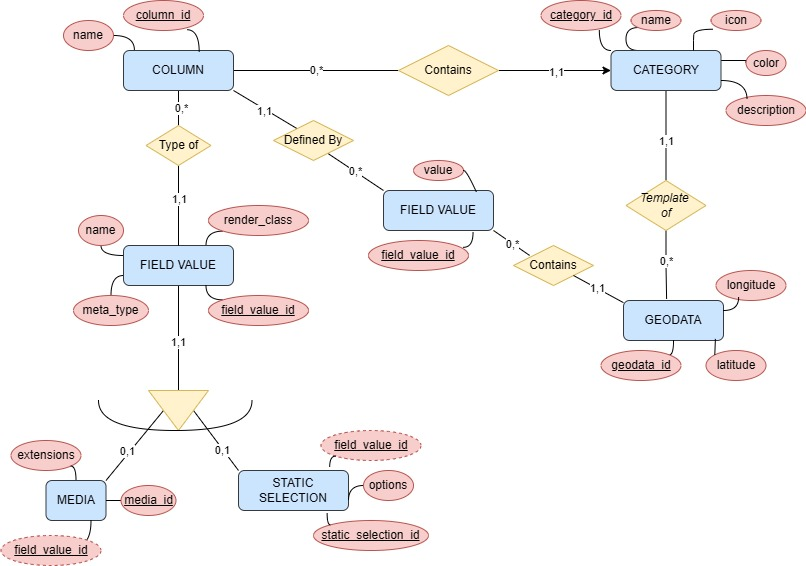
\includegraphics[width=0.8\textwidth]{images/old_merx.jpg}
\caption{Modelo de datos original de GeoBase}
\label{fig:oldmerx}
\end{figure}


En otras palabras, el modelo establece relaciones directas entre \textbf{Geodata}, \textbf{Column} y \textbf{FieldValue}, pero no incluye mecanismos para que un valor pueda ser a la vez un contenedor de otros valores anidados. Esta falta de soporte para estructuras recursivas o jerárquicas impide representar formularios con campos compuestos o grupos de campos que dependan unos de otros, lo cual es esencial para manejar formularios anidados o dinámicos con múltiples niveles de profundidad.

Por tanto, aunque los tipos de datos básicos y multimedia pueden ser almacenados y gestionados con el esquema actual, la ausencia de una relación que permita anidar campos o valores limita la capacidad del sistema para representar estructuras complejas de datos. Para superar esta restricción, es necesario rediseñar el modelo incorporando una nueva entidad, denominada \textbf{Form}, que funcionará como un nuevo \textbf{FieldType} para las columnas. Al igual que \textbf{Category}, esta entidad se relacionará con \textbf{Column}, permitiendo así la recursividad necesaria para representar formularios anidados. Esta propuesta se ilustra en la Figura \ref{fig:newmerx}.

\begin{figure}[H]
\centering
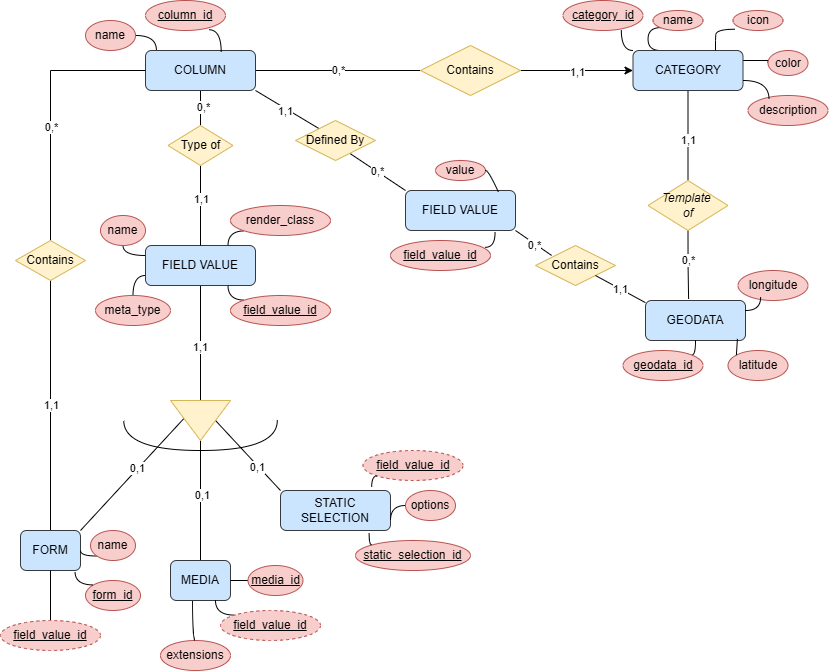
\includegraphics[width=0.8\textwidth]{images/new_merx.png}
\caption{Propuesta de modelo de datos para GeoBase}
\label{fig:newmerx}
\end{figure}

El modelo de datos actualizado introduce una estructura jerárquica para formularios mediante la implementación de nuevas entidades y modificaciones en las relaciones existentes. Como se observa en el MERX actualizado (Figura \ref{fig:newmerx}), la entidad \textbf{Form} se integra como componente fundamental para permitir anidamiento de campos. Esta entidad se define a partir de las siguientes propiedades:

\begin{itemize}
  \item form\_id (\textbf{PK}): Valor entero que identifica de forma única una fila de esta tabla.
  \item field\_type\_id (\textbf{FK}, heredado): Valor entero que identifica de forma única una fila de la tabla \textit{FieldType} (de la cual esta tabla hereda). 
  \item name: Texto utilizado para nombrar el tipo de campo.
\end{itemize}

La relación con la entidad \textbf{Column} se modifica para permitir una dualidad estructural, donde cada columna puede pertenecer tanto a una categoría como a un formulario anidado.

\begin{itemize}
  \item column\_id (\textbf{PK}): Valor entero que identifica de forma única una fila de esta tabla.
  \item form\_id (\textbf{FK}, opcional): Valor entero que identifica de forma única una fila de la tabla \textit{Form}; este campo puede contener valores nulos.
  \item category\_id (\textbf{FK}, opcional): Valor entero que identifica de forma única una fila de la tabla \textit{Category}; este campo puede contener valores nulos.
  \item  field\_type\_id (\textbf{FK}): Valor entero que identifica de forma única una fila de la tabla \textit{FieldType}.
  \item name: Texto utilizado para nombrar el tipo de campo.
\end{itemize}

La integración con el sistema existente se realiza mediante el mecanismo de tipos de campo \textbf{FieldType}, donde cada formulario se registra como un \texttt{meta\_type} específico. Esta aproximación permite mantener la coherencia del sistema original mientras se añade capacidad de composición jerárquica. El campo \texttt{field\_type\_id} en la entidad \textbf{Form} establece una relación de dependencia con \textbf{FieldType}, permitiendo que los formularios hereden las propiedades base de los tipos de campo y puedan ser procesados por el motor de renderizado especializado (\texttt{FORM\_RENDER\_CLASS}).

La estructura resultante soporta anidamiento recursivo mediante la relación entre \textbf{Form} y \textbf{Column}, donde un formulario puede contener múltiples columnas que a su vez pueden hacer referencia a otros formularios. Este diseño se alinea con los principios de composición en sistemas complejos descritos en la literatura especializada, particularmente en lo concerniente a la mantenibilidad y extensibilidad de estructuras de datos jerárquicas. La regla de eliminación en cascada (DeleteRule.CASCADE) garantiza la integridad referencial al eliminar elementos padre en la jerarquía.

\section{Arquitectura}

La arquitectura de la aplicación se mantuvo bajo el enfoque de Clean Architecture (\cite{martin2017}), preservando la separación en capas y los principios de independencia entre dominio, datos y presentación. Esta decisión se fundamenta en la robustez y flexibilidad que ofrece este patrón, ampliamente recomendado en la literatura especializada para el desarrollo de sistemas mantenibles y escalables. La estructura general del proyecto y las dependencias entre capas se observan en la Figura \ref{fig:cleanarquitecturecode} y la Figura \ref{fig:cleanarquitecturedependences}, respectivamente.

\begin{figure}[H]
  \centering
  \begin{minipage}[b]{0.4\textwidth}
    \centering
    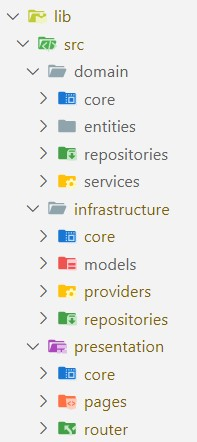
\includegraphics[width=\textwidth]{images/clean_arq_code_structure.jpg}
    \caption{Estructura en código de Clean Arquitecture.}
    \label{fig:cleanarquitecturecode}
  \end{minipage}
  \hspace{0.02\textwidth}
  \begin{minipage}[b]{0.4\textwidth}
    \centering
    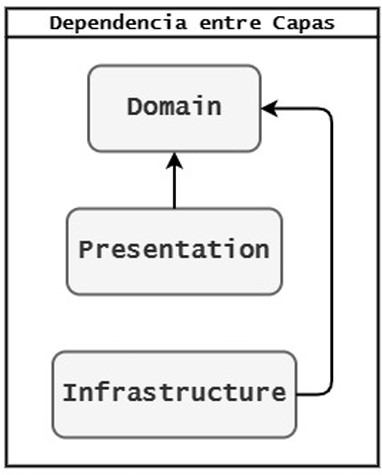
\includegraphics[width=\textwidth]{images/clean_arq_dependences.jpg}
    \caption{Diagrama de dependencia entre capas.}
    \label{fig:cleanarquitecturedependences}
  \end{minipage}
  \label{fig:mer_comparacion}
\end{figure}

Si bien no se modificó la arquitectura fundamental, se realizaron extensiones en todas las capas para dar soporte a las nuevas funcionalidades de Geobase. En particular, fue necesario actualizar las clases relacionadas con la entidad \textbf{Column}, ya que hasta el momento cada columna requería la propiedad \texttt{category\_id}. Con la introducción de los formularios, se permitió que una columna pertenezca tanto a una categoría como a un formulario; por lo tanto, tanto \texttt{category\_id} como \texttt{form\_id} pasaron a ser opcionales, brindando mayor flexibilidad en la definición de la estructura de los formularios.

En la capa de dominio, se incorporaron dos nuevas entidades fundamentales: \texttt{FieldTypeFormGetEntity} y \texttt{FieldTypeFormPostEntity}. La primera, como se ilustra en la Figura \ref{fig:fieldtypeformgetentity}, extiende la funcionalidad de \texttt{FieldTypeGetEntity} e introdujo una colección de columnas asociadas, permitiendo así la representación de formularios que agrupen múltiples campos estructurados. Por su parte, \texttt{FieldTypeFormPostEntity}, mostrada en la Figura \ref{fig:fieldtypeformpostentity}, está orientada a la creación y envío de formularios, integrando también una lista de columnas como atributo principal. Ambas clases serán diseñadas para facilitar la conversión a formato JSON y su construcción a partir de dicho formato, lo cual resultará esencial para las funcionalidades relacionadas con la exportación e importación de datos.

\begin{figure}[H]
  \centering
  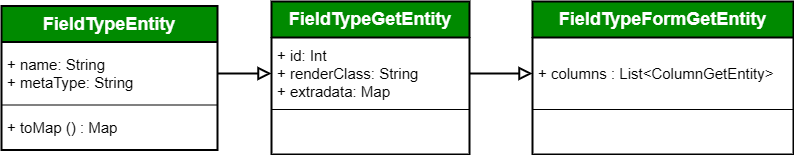
\includegraphics[width=\textwidth]{images/fieldtypeform_get_entity.png}
  \caption{Estructura de la clase \texttt{FieldTypeFormGetEntity}.}
  \label{fig:fieldtypeformgetentity}
\end{figure}

\begin{figure}[H]
  \centering
  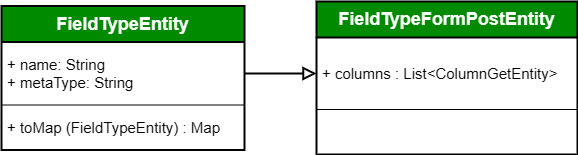
\includegraphics[width=0.65\textwidth]{images/fieldtypeform_post_entity.png}
  \caption{Estructura de la clase \texttt{FieldTypeFormPostEntity}.}
  \label{fig:fieldtypeformpostentity}
\end{figure}

Siguiendo en la capa del dominio, se añadió una nueva interfaz de repositorio, \texttt{IFieldTypeFormRepository} (Figura \ref{fig:iformrepo}), la cual define las operaciones fundamentales para la gestión de formularios, tales como la carga, creación y eliminación de entidades de formulario. Esta interfaz es implementada por el servicio \texttt{FieldTypeFormService} (Figura \ref{fig:formservice}), que actúa como intermediario entre la lógica de dominio y la fuente de datos, encapsulando la lógica de acceso y manipulación de los formularios.

\begin{figure}[H]
  \centering
  \begin{minipage}[b]{0.45\textwidth}
    \centering
    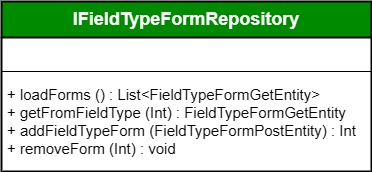
\includegraphics[width=\textwidth]{images/iform_repo.jpg}
    \caption{Interface del repositorio de la entidad \textbf{Form}}
    \label{fig:iformrepo}
  \end{minipage}
  \hspace{0.02\textwidth}
  \begin{minipage}[b]{0.45\textwidth}
    \centering
    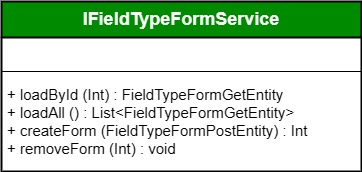
\includegraphics[width=\textwidth]{images/iformservice.jpg}
    \caption{Interface del servicio de la entidad \textbf{Form}}
    \label{fig:formservice}
  \end{minipage}
\end{figure}

En la capa de Infraestructura se implementaron los modelos correspondientes a los formularios, específicamente las clases \texttt{FieldTypeFormGetModel} y \texttt{FieldTypeFormPostModel}. Estas clases son responsables de representar los datos en las operaciones de lectura (GET) y escritura (POST), respectivamente. Además, se desarrolló una extensión que permite convertir estos modelos a sus respectivas entidades de dominio, facilitando así la integración entre capas y asegurando la coherencia en la transformación de datos.

\begin{figure}[H]
  \centering
  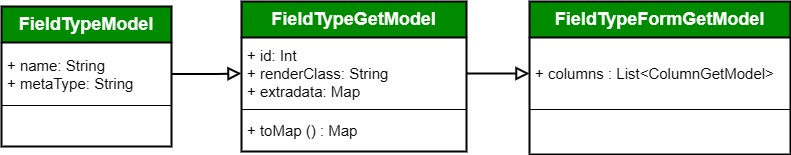
\includegraphics[width=1.0\textwidth]{images/form_get_model.jpg}
  \caption{Modelo GET de la entidad \textbf{Form}}
  \label{fig:formgetmodel}
\end{figure}
\begin{figure}[H]
    \centering
    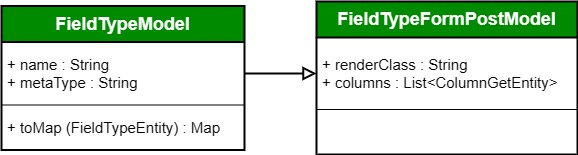
\includegraphics[width=0.8\textwidth]{images/form_post_model.jpg}
    \caption{Modelo POST de la entidad \textbf{Form}}
    \label{fig:formpostmodel}
\end{figure}

Se agregó la interface \texttt{IFieldTypeFormProvider} (Figura \ref{fig:iformprovider}) con su respectiva implementación. Hubo modificaciones también en otras clases para garantizar la consistencia con los formularios, como es el caso de la clase \texttt{ColumnProvider}, a la cual se le adicionó el método \texttt{getAllFromForm} como vemos en su interface (Figura \ref{fig:icolumnprovider})

\begin{figure}[H]
  \centering
  \begin{minipage}[b]{0.43\textwidth}
    \centering
    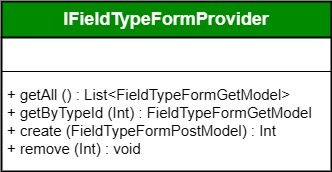
\includegraphics[width=\textwidth]{images/form_provider.jpg}
    \caption{Interface de la clase \texttt{FieldTypeFormProvider}}
    \label{fig:iformprovider}
  \end{minipage}
  \hspace{0.02\textwidth}
  \begin{minipage}[b]{0.47\textwidth}
    \centering
    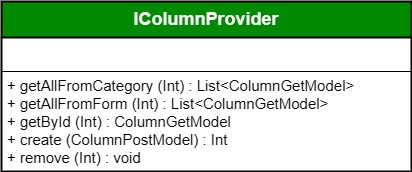
\includegraphics[width=\textwidth]{images/column_provider.jpg}
    \caption{Interface de la clase \texttt{ColumnProvider}}
    \label{fig:icolumnprovider}
  \end{minipage}
\end{figure}

En la capa de Presentación se proyectó la organización y desarrollo de las vistas necesarias para la gestión de formularios, así como la ampliación de las funcionalidades asociadas a las entidades \textbf{Geodata} y \textbf{Category}. Se contempló la creación de un directorio específico para las vistas de formularios (Figura \ref{fig:formpage}), lo que permite centralizar y estructurar de manera eficiente todos los componentes visuales y lógicos relacionados con la interacción del usuario en torno a los formularios.

Adicionalmente, se incorporaron nuevos métodos y componentes en las vistas correspondientes a \textbf{Geodata} y \textbf{Category} (Figuras \ref{fig:geodatapage} y \ref{fig:categorypage}), con el objetivo de habilitar operaciones avanzadas como la exportación e importación de datos. Esta organización modular ya estaba aplicada en Geobase desde su desarrollo y facilita la escalabilidad del sistema, permitiendo que cada entidad cuente con su propio conjunto de páginas, widgets y bloques lógicos (BLoC/Cubit), distribuidos en subdirectorios que reflejan claramente las responsabilidades de cada componente.

\begin{figure}[H]
  \centering
  \begin{minipage}[b]{0.32\textwidth}
    \centering
    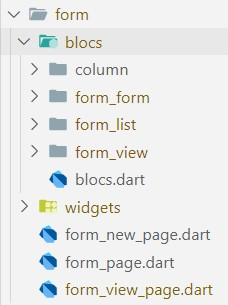
\includegraphics[width=0.7\textwidth]{images/form_page.jpg}
    \caption{Directorio de las vistas de \textbf{Form}}
    \label{fig:formpage}
  \end{minipage}
  \hspace{0.02\textwidth}
  \begin{minipage}[b]{0.3\textwidth}
    \centering
    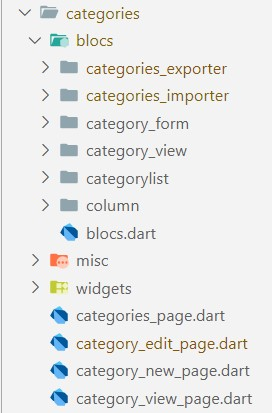
\includegraphics[width=\textwidth]{images/category_page.jpg}
    \caption{Directorio de las vistas de \textbf{Category}}
    \label{fig:categorypage}
  \end{minipage}
  \hspace{0.02\textwidth}
  \begin{minipage}[b]{0.3\textwidth}
    \centering
    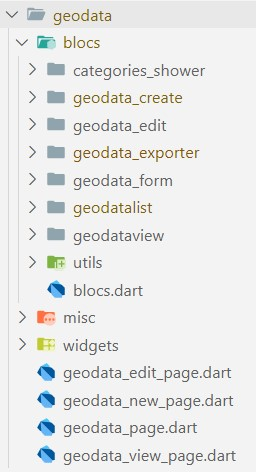
\includegraphics[width=\textwidth]{images/goedata_page.jpg}
    \caption{Directorio de las vistas de \textbf{Geodata}}
    \label{fig:geodatapage}
  \end{minipage}
\end{figure}

Para la renderización de las columnas tanto en categorías como en formularios, se realizó la configuración y reutilización de un conjunto de clases especializadas, que permiten gestionar de manera uniforme tanto la entrada de datos como la visualización de los registros ya creados. Esta decisión responde a la necesidad de soportar formularios con estructura anidada, ya que dichos formularios podrán se incluyen dentro de los mismos tipos de columnas que previamente solo se utilizaban en el contexto de categorías.

La nueva organización contempla la utilización de directorios específicos para los distintos aspectos de la interfaz de usuario relacionados con los campos de las columnas. Por un lado, el directorio \texttt{field\_view\_widgets} contiene los componentes responsables de la visualización de los diferentes tipos de campos (Figura \ref{fig:fieldviews}). Por otro lado, el directorio \texttt{field\_input\_widgets} agrupa los widgets encargados de la captura de datos para cada tipo de columna (Figura \ref{fig:fieldinputs}). Finalmente, el directorio \texttt{field\_render\_classes}, dentro de \texttt{render\_classes}, alberga las clases de renderizado que definen la lógica específica para la presentación y gestión de cada tipo de campo (Figura \ref{fig:fieldrender}).

\begin{figure}[H]
  \centering
  \begin{minipage}[b]{0.3\textwidth}
    \centering
    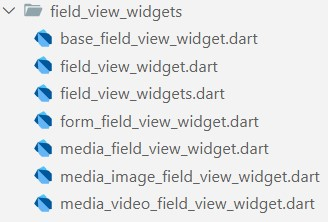
\includegraphics[width=\textwidth]{images/field_views.jpg}
    \caption{Directorio de los \textit{views} de los tipos de columnas}
    \label{fig:fieldviews}
  \end{minipage}
  \hspace{0.02\textwidth}
  \begin{minipage}[b]{0.3\textwidth}
    \centering
    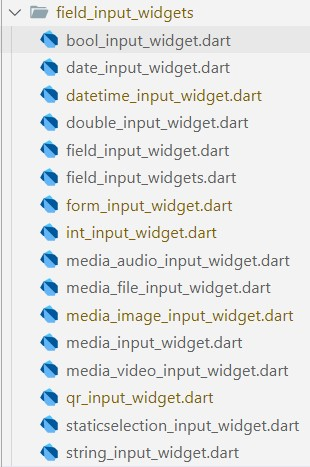
\includegraphics[width=\textwidth]{images/field_inputs.jpg}
    \caption{Directorio de los \textit{inputs} de los tipos de columnas.}
    \label{fig:fieldinputs}
  \end{minipage}
  \hspace{0.02\textwidth}
  \begin{minipage}[b]{0.3\textwidth}
    \centering
    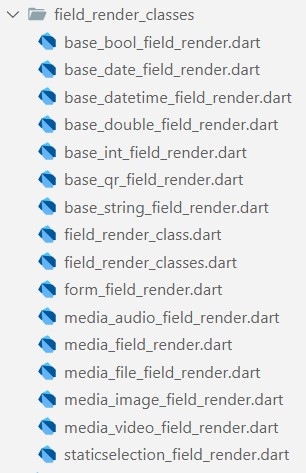
\includegraphics[width=\textwidth]{images/field_renders.jpg}
    \caption{Directorio de los \textit{renders} de los tipos de columnas}
    \label{fig:fieldrender}
  \end{minipage}
\end{figure}

Como parte de la ampliación de los tipos de datos en el sistema, se incorporaron campos para códigos QR, clasificados como tipo base, así como campos para video, que se gestionan como tipo Media. Estas nuevas opciones permiten ampliar la funcionalidad de los formularios y categorías, facilitando la integración de datos codificados y contenido audiovisual. Los detalles específicos de su implementación y uso serán abordados en secciones posteriores del documento.

\section{Tecnologías utilizadas}

En primer lugar, se incluyó la dependencia record (\cite{record2024}), la cual permite implementar la funcionalidad de grabación de audio directamente desde la aplicación. La integración de esta tecnología hace posible que los usuarios puedan, mediante una interfaz sencilla, iniciar y detener grabaciones asociada a los formularios o categorías.

Asimismo, se contempló la integración de la dependencia excel (\cite{excel2024}), destinada a la generación y manipulación de archivos en formato Excel. Esta funcionalidad resulta esencial para la exportación y manejo estructurado de grandes volúmenes de datos, permitiendo su análisis posterior en herramientas ofimáticas. 

Por otro lado, se añadió la dependencia qr\_code\_scanner (\cite{qrcodescanner2024}), la cual habilita el escaneo de códigos QR mediante la cámara del dispositivo. Esta capacidad facilita la vinculación rápida de información y la identificación de elementos en campo, optimizando los procesos de registro y consulta.

Finalmente, se consideró la inclusión de la dependencia path (\cite{path2024}), que proporciona utilidades para la manipulación eficiente de rutas y archivos en el sistema de almacenamiento del dispositivo.


\section{Detalles de implementación}

En este capítulo se presentan las funcionalidades desarrolladas para la gestión avanzada de datos en GeoBase, enfocándose en la implementación de formularios anidados, así como en los procesos de importación de categorías y exportación de geodata. Se describen los componentes técnicos y las estrategias utilizadas para garantizar una interacción flexible y eficiente con los datos, manteniendo la coherencia y escalabilidad del sistema.

\subsection{Formularios anidados}

En el diseño propuesto, una columna de tipo formulario permite al usuario gestionar en tiempo de ejecución una lista de subformularios, todos ellos con la misma estructura. Esto significa que, en lugar de contener un único conjunto de campos, este tipo de columna puede almacenar múltiples instancias del mismo formulario, facilitando así la captura y edición de bloques de datos homogéneos según las necesidades del usuario.

La implementación se basa en un widget especializado denominado \texttt{FormFieldInputWidget} (Firgura \ref{fig:forminput}), encargado de determinar si el formulario se encuentra en modo de creación o edición, y según corresponda, efectuar la visualización y gestión de la lista de subformularios. Si el formulario está en modo creación, se inicializa una lista vacía; en modo edición, se deserializan los valores previamente almacenados y se cargan como valores iniciales.

\begin{figure}[H]
  \centering
  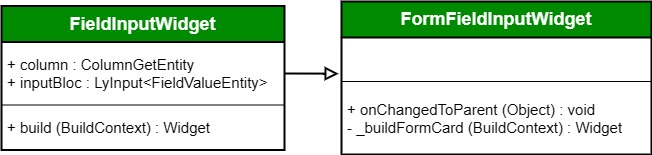
\includegraphics[width=0.9\textwidth]{images/form_field_input.jpg}
  \caption{Clase para construir entrada de formularios anidados}
  \label{fig:forminput}
\end{figure}

Cada subformulario es representado como una tarjeta expandible, que contiene los campos definidos en la configuración original. Esta estructura permite al usuario agregar o eliminar instancias de subformularios de manera dinámica, garantizando flexibilidad y control sobre la información ingresada. El estado de la lista es gestionado por un \texttt{Cubit} específico, denominado \texttt{DynamicFormCubit} (Figura \ref{fig:dynamicformlist}), responsable de manejar las operaciones de creación y eliminación de subformularios.

\begin{figure}[H]
  \centering
  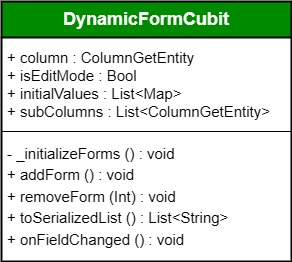
\includegraphics[width=0.5\textwidth]{images/dynamic_form_list.jpg}
  \caption{\texttt{Cubit} para administrar el widget \texttt{FormFieldInputWidget}}
  \label{fig:dynamicformlist}
\end{figure}

Los datos ingresados en estos subformularios se serializan como una lista de mapas en formato JSON, lo que permite su almacenamiento eficiente y su reconstrucción durante la edición. Para mantener la coherencia con el resto del sistema, estos valores se encapsulan en objetos del tipo \texttt{FieldValuePostEntity} o \texttt{FieldValuePutEntity}, según el caso.


\subsection{Importación de categorías}

La funcionalidad de importación de categorías se implementó mediante un componente dedicado basado en un \texttt{Cubit}, denominado \texttt{CategoriesImporterCubit} (Figura \ref{fig:categoryimporter}). Este componente gestiona el flujo completo de importación, desde la selección del archivo hasta la creación de las entidades correspondientes en la base de datos de la aplicación.

\begin{figure}[H]
  \centering
  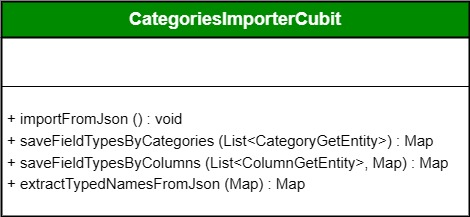
\includegraphics[width=0.7\textwidth]{images/category_importer.jpg}
  \caption{\texttt{Cubit} para importar categorías}
  \label{fig:categoryimporter}
\end{figure}

El proceso inicia solicitando al usuario la selección de un archivo en formato JSON, el cual debe contener la estructura serializada de las categorías a importar. Para ello, se utiliza la biblioteca \texttt{file\_picker}, que permite abrir un diálogo de selección de archivos y restringir la elección a archivos con la extensión adecuada.

La importación de las entidades se realiza de manera recursiva, comenzando por los tipos de campo asociados a cada categoría (incluyendo formularios anidados y selecciones estáticas), y posteriormente creando las categorías propiamente dichas. Para cada tipo de campo o categoría, se utilizan los servicios de dominio existentes, asegurando así la integridad y consistencia de los datos importados.

Se implementó un manejo robusto de errores y estados, informando al usuario sobre el progreso, éxito o posibles fallos durante el proceso de importación. Esto facilitará tanto la experiencia de uso como el diagnóstico de problemas en caso de incidencias.

\subsection{Exportación de geodata}

La funcionalidad de exportación de \textit{geodata} está gestionada por un componente específico basado en un \texttt{Cubit}, denominado \texttt{GeodataExporterCubit} (Figura \ref{fig:geodataexporter}). Este componente es responsable de todo el flujo de exportación, desde la obtención de los datos hasta la generación y almacenamiento del archivo final.

\begin{figure}[H]
  \centering
  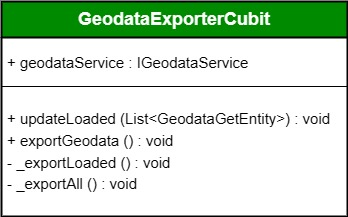
\includegraphics[width=0.7\textwidth]{images/geodata_exporter.jpg}
  \caption{\texttt{Cubit} para exportar \textit{geodata}}
  \label{fig:geodataexporter}
\end{figure}

El proceso comienza con la carga de los registros de geodata, que pueden ser seleccionados previamente o recuperados en su totalidad mediante el servicio de dominio correspondiente. Una vez cargados los datos, el sistema permite al usuario exportarlos en formato Excel, estructurando la información en hojas separadas según las categorías y formularios presentes en el sistema.

Durante la generación del archivo Excel, se crean encabezados dinámicos que reflejan la estructura de los datos, incluidos los campos básicos y los formularios anidados. Para cada registro, se procesan los campos de tipo formulario de manera recursiva, generando hojas adicionales para los subformularios y manteniendo referencias cruzadas mediante identificadores únicos. Los campos de tipo Media, como imágenes o videos, son tratados especialmente: el archivo Excel contiene referencias a los archivos multimedia, que son copiados a una carpeta específica dentro del directorio de exportación, asegurando así la integridad y portabilidad del conjunto de datos exportado.

El usuario selecciona el destino de la exportación a través de un diálogo de selección de carpeta. El sistema crea un directorio exclusivo para la exportación, incluyendo tanto el archivo Excel como una subcarpeta para los archivos multimedia asociados. Los nombres de los archivos y carpetas incorporan marcas de tiempo para evitar sobrescrituras y facilitar la organización.

El sistema contempla un manejo robusto de errores y estados, informando al usuario sobre el avance, éxito o posibles incidencias durante el proceso de exportación. Esta retroalimentación es fundamental para garantizar una experiencia de usuario clara y confiable.


\chapter{Caso de estudio}

El caso de estudio se centra en la recopilación de datos en campo realizada por una empresa eléctrica en zonas rurales, donde la necesidad de registrar información precisa y estructurada sobre el estado de la infraestructura eléctrica es crítica para optimizar el mantenimiento y garantizar un suministro eficiente.

La problemática principal radica en la complejidad de gestionar datos heterogéneos y estructurados, como los relacionados con postes eléctricos y transformadores, organizados en categorías y subcategorías específicas (por ejemplo, “Datos generales”, “Estado” y “Acciones requeridas”). Además, la inclusión de datos multimedia —fotos, videos y notas de voz— resulta fundamental para documentar daños y condiciones en terreno. La aplicación debe además permitir la georreferenciación precisa de cada punto registrado y facilitar la exportación de la información para su posterior análisis mediante algoritmos de optimización de rutas, con el fin de priorizar reparaciones urgentes y reducir tiempos y costos.

La figura~\ref{fig:casoestudio} ilustra un modelo de entidades y sus relaciones para realizar pruebas a las nuevas funcionalidades implementadas. En este modelo, el \textit{Poste de luz} constituye la entidad principal, permitiendo registrar atributos esenciales como la altura y el material del poste. Cada poste puede estar asociado a uno o varios transformadores, reflejando la realidad operativa donde un mismo soporte físico puede albergar distintos equipos eléctricos.

La entidad \textit{Transformador} almacena información específica de cada equipo, incluyendo un código identificador, que puede ser capturado mediante un código QR para agilizar la trazabilidad en campo, y registros de audio que documentan el nivel de ruido, útil para diagnóstico preventivo. Además, cada transformador puede tener múltiples registros de \textit{Mantenimiento}, lo que permite llevar un historial detallado de las intervenciones técnicas realizadas a lo largo del tiempo.

Cada registro de mantenimiento vinculado a un transformador contiene datos como la fecha de la intervención, archivos multimedia (video e imagen) que evidencian el estado del equipo, y la factura correspondiente al servicio realizado. Esta estructura jerárquica y anidada facilita la organización, consulta y análisis de la información recolectada, asegurando la trazabilidad de cada elemento de la infraestructura eléctrica y optimizando los procesos de mantenimiento en zonas rurales.

\begin{figure}[H]
  \centering
  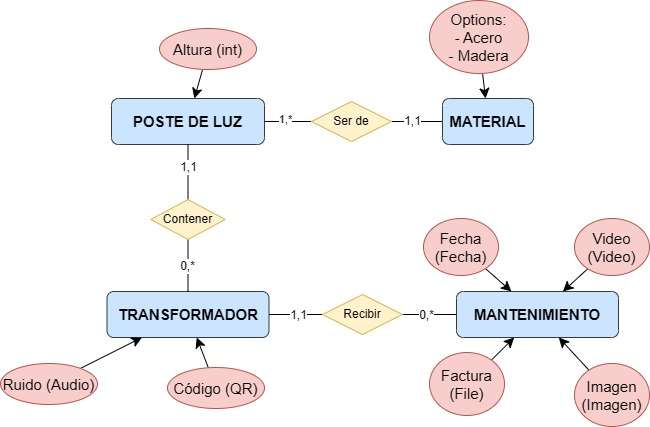
\includegraphics[width=0.7\textwidth]{images/functionality_test/caso_estudio.jpg}
  \caption{\textit{MERX} del las entidades para probar las funcionalidades acorde al caso de estudio}
  \label{fig:casoestudio}
\end{figure}

Para llevar a cabo las pruebas funcionales, se utilizó un dispositivo móvil con las siguientes características técnicas:

\begin{itemize}
    \item \textbf{Modelo del dispositivo:} Nokia G10.
    \item \textbf{Sistema operativo:} Android™ 11 (actualizable a versiones posteriores, dependiendo de la disponibilidad).
    \item \textbf{Memoria RAM:} 3 GB
    \item \textbf{Almacenamiento interno:} 32 GB
\end{itemize}

A continuación, se describen las pruebas realizadas, orientadas a validar cada uno de los objetivos específicos de la tesis y su ajuste al contexto real y particular de la recopilación de datos en campo por parte de la empresa eléctrica en zonas rurales, siguiendo un orden cronológico que refleja el flujo natural de uso de la aplicación:


\section{Prueba 1: Carga de la definición de categorías desde JSON.}
\begin{itemize}
    \item \textit{Objetivo:} Verificar que la aplicación pueda importar correctamente la estructura de categorías y subcategorías definidas para el caso de estudio.
    \item \textit{Entrada:} Archivo JSON con la definición de categorías, subcategorías y tipos de campo asociados.
    \item \textit{Salida esperada:} Las categorías y sus formularios asociados se cargan sin errores y se reflejan correctamente en la interfaz.
\end{itemize}

El flujo inicial de la aplicación comienza con la visualización de la página de categorías en un estado vacío, tal como se muestra en la Figura \ref{fig:loadcategories1}. En esta etapa, no se ha cargado aún ninguna definición de categorías, por lo que la interfaz presenta un listado vacío, esperando la importación de datos.

A continuación, se procede a cargar el archivo JSON que contiene la definición estructurada de las categorías y sus formularios asociados. Tras completar esta acción, la página de categorías se actualiza para reflejar la información importada, como se observa en la Figura \ref{fig:loadcategories2}. En esta vista, las categorías ya aparecen listadas, mostrando que la carga fue exitosa y que la aplicación ha procesado correctamente la estructura del archivo.

Finalmente, la Figura \ref{fig:loadcategories3} ilustra cómo, a partir de las categorías cargadas, se generan automáticamente los formularios correspondientes. Estos formularios están disponibles para su utilización en la captura de datos, evidenciando que la aplicación ha integrado correctamente la información importada y está lista para su uso en campo.

\begin{figure}[H]
  \centering
  \begin{minipage}[b]{0.3\textwidth}
    \centering
    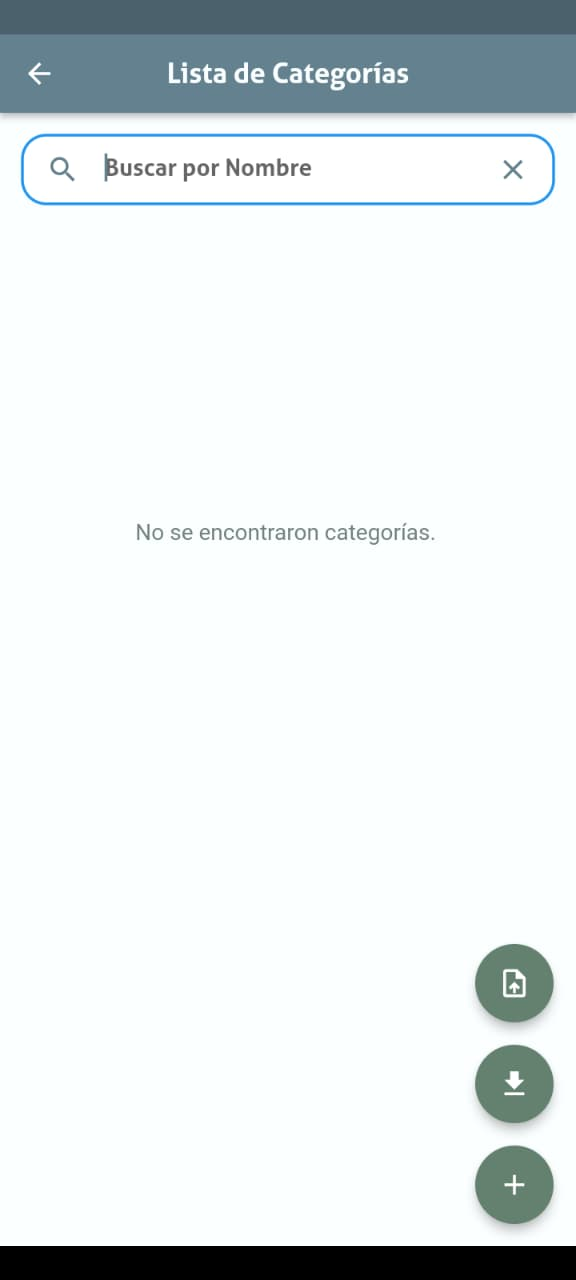
\includegraphics[width=\textwidth]{images/functionality_test/load_categories_1.jpg}
    \caption{Página de categorías antes de cargar del \textit{JSON}}
    \label{fig:loadcategories1}
  \end{minipage}
  \hspace{0.02\textwidth}
  \begin{minipage}[b]{0.3\textwidth}
    \centering
    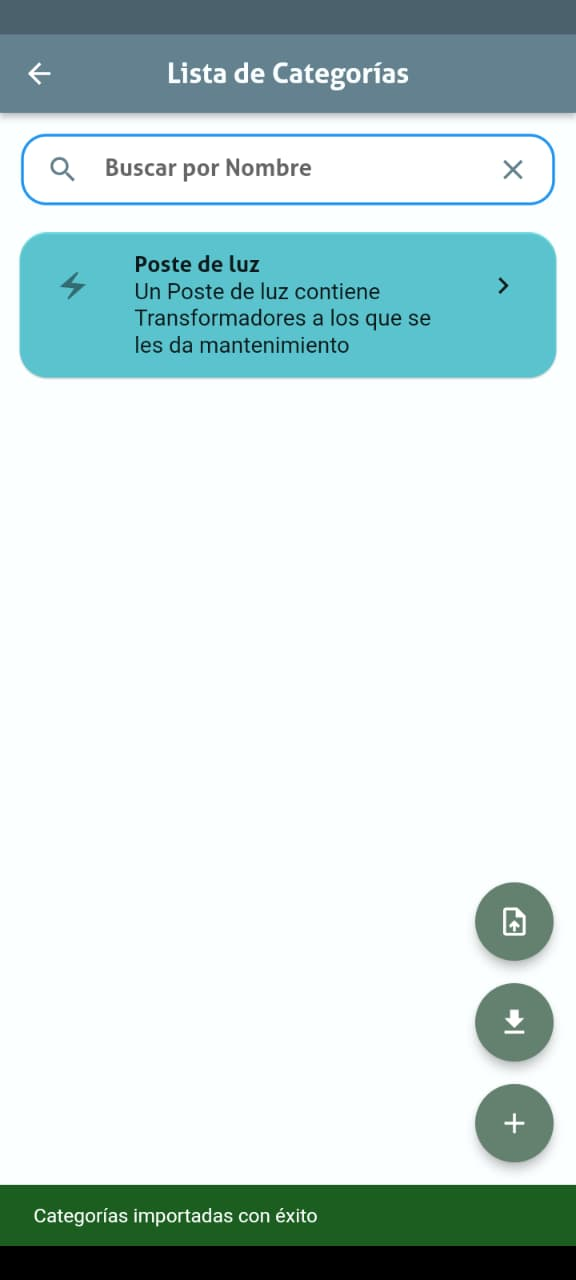
\includegraphics[width=\textwidth]{images/functionality_test/load_categories_2.jpg}
    \caption{Página de categorías después de cargar del JSON}
    \label{fig:loadcategories2}
  \end{minipage}
  \hspace{0.02\textwidth}
  \begin{minipage}[b]{0.3\textwidth}
    \centering
    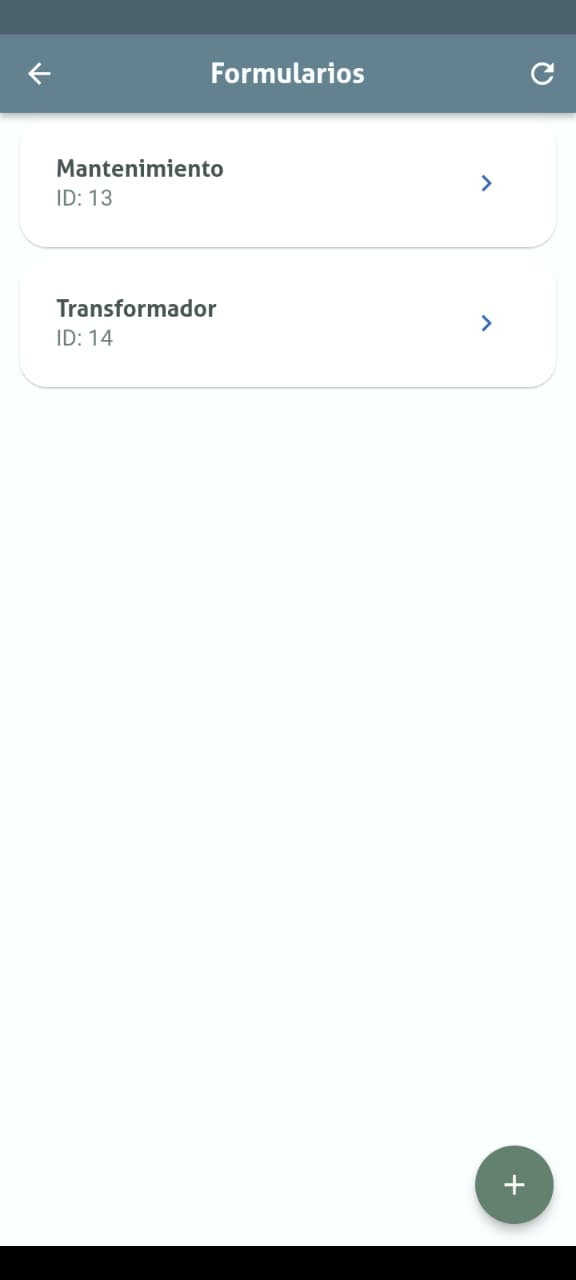
\includegraphics[width=\textwidth]{images/functionality_test/load_categories_3.jpg}
    \caption{Formularios creados al cargar las categorías del JSON}
    \label{fig:loadcategories3}
  \end{minipage}
\end{figure}

\section{Prueba 2: Renderizado de formularios anidados.}
\begin{itemize}
  \item \textbf{Objetivo:} Confirmar que, dado un punto georreferenciado perteneciente a una categoría con formularios anidados, la aplicación despliega correctamente dichos formularios para la captura de datos.
  \item \textbf{Entrada:} Selección de un punto en el mapa con categoría asignada.
  \item \textbf{Salida esperada:} Visualización dinámica del formulario anidado correspondiente, con posibilidad de agregar múltiples subformularios.
\end{itemize}

El proceso de renderizado de formularios anidados comienza con la selección de un punto georreferenciado en el mapa que pertenece a una categoría específica, como se muestra en la Figura \ref{fig:geodataview1}. En esta primera vista, los formularios asociados a dicho punto se presentan en un estado contraído, lo que permite al usuario tener una visión general y ordenada de la información disponible sin saturar la pantalla. Esta presentación inicial facilita la navegación y la identificación rápida de los formularios relacionados.

Al interactuar con los formularios, la aplicación despliega dinámicamente el contenido anidado, expandiendo los formularios para mostrar los campos y subformularios correspondientes, tal como se observa en la Figura \ref{fig:geodataview2}. Esta expansión permite al usuario ingresar datos detallados y agregar múltiples subformularios según sea necesario, confirmando que la aplicación maneja correctamente la estructura jerárquica de los formularios. De esta manera, se garantiza una experiencia fluida y funcional para la captura de datos complejos dentro de un mismo punto georreferenciado.

\begin{figure}[H]
  \centering
  \begin{minipage}[b]{0.3\textwidth}
    \centering
    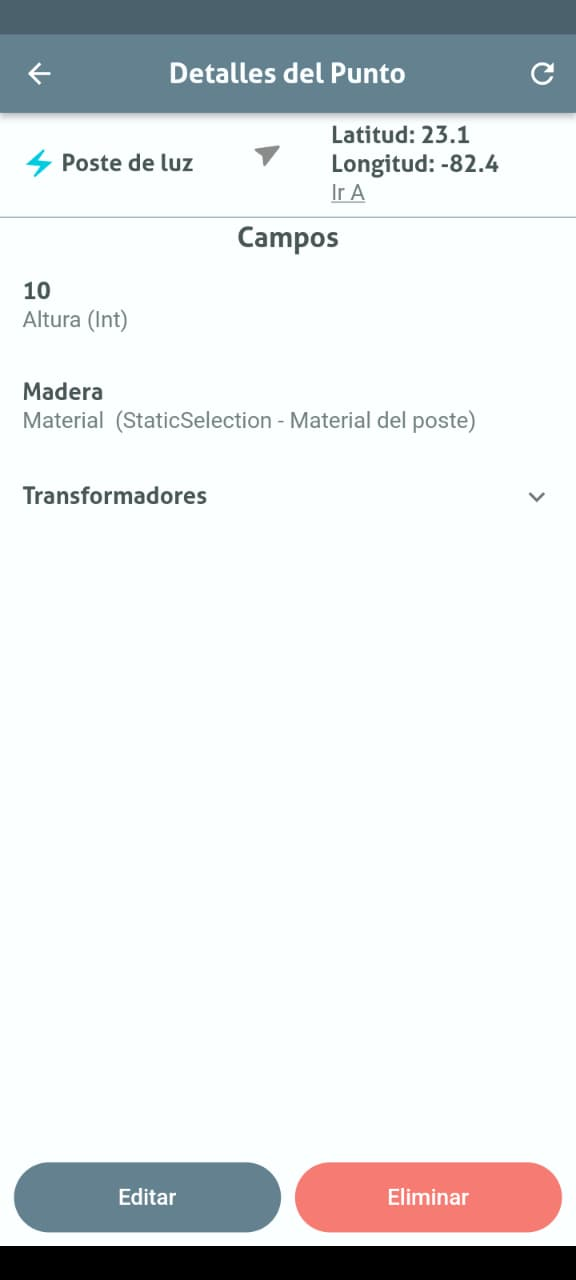
\includegraphics[width=\textwidth]{images/functionality_test/geodata_view1.jpg}
    \caption{Página de visualización de \textit{geodata}. Formularios contraídos}
    \label{fig:geodataview1}
  \end{minipage}
  \hspace{0.02\textwidth}
  \begin{minipage}[b]{0.3\textwidth}
    \centering
    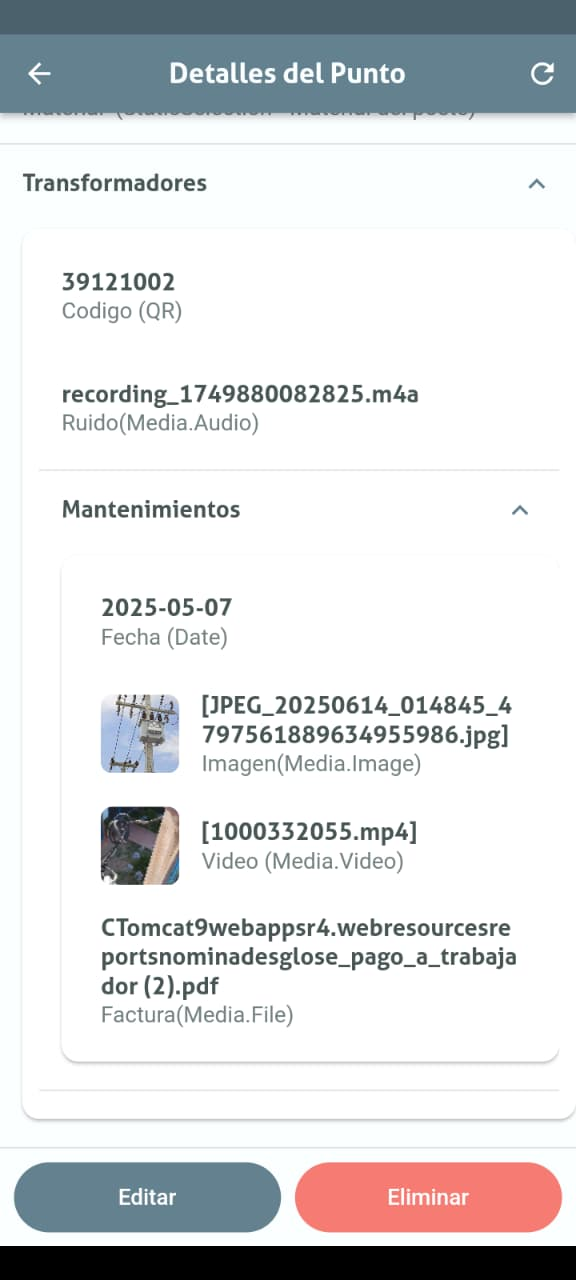
\includegraphics[width=\textwidth]{images/functionality_test/geodata_view2.jpg}
    \caption{Página de visualización de \textit{geodata}. Formularios expandidos}
    \label{fig:geodataview2}
  \end{minipage}
\end{figure}

\section{Prueba 3: Captura de datos multimedia y códigos QR en formularios.}
\begin{itemize}
  \item \textit{Objetivo:} Validar la funcionalidad de las columnas especializadas para ingresar datos multimedia (fotos, videos, notas de voz) y códigos QR dentro de los formularios anidados.
  \item \textit{Entrada:} Ingreso de datos en las columnas correspondientes durante la edición del formulario.
  \item \textit{Salida esperada:} Los datos multimedia y códigos QR se capturan correctamente, se almacenan y pueden ser visualizados o escaneados según corresponda.
\end{itemize}

El proceso de captura de códigos QR inicia con la interacción del usuario para escanear un código directamente desde la aplicación, como se aprecia en la Figura \ref{fig:medias1}. En esta etapa, la interfaz habilita el uso de la cámara para reconocer el código, permitiendo que el sistema reciba la información codificada y la asocie al formulario correspondiente. Posteriormente, una vez que el código QR ha sido capturado, la aplicación muestra la visualización del mismo, tal como se observa en la Figura \ref{fig:medias2}. Esta visualización confirma que el dato fue almacenado correctamente y está disponible para su consulta o para ser utilizado en procesos posteriores.

Con respecto a los campos de tipo audio, imagen o video, inicialmente se consulta al usuario desde donde quiere cargar el dato (desde el dispositivo o capturarlo desde la aplicación en el momento) y luego se previsualiza como una miniatura en el caso de las imagenes o videos. La Figura \ref{fig:medias3} presenta las opciones que el usuario tiene para cargar un video dentro del formulario.

\begin{figure}[H]
  \centering
  \begin{minipage}[b]{0.3\textwidth}
    \centering
    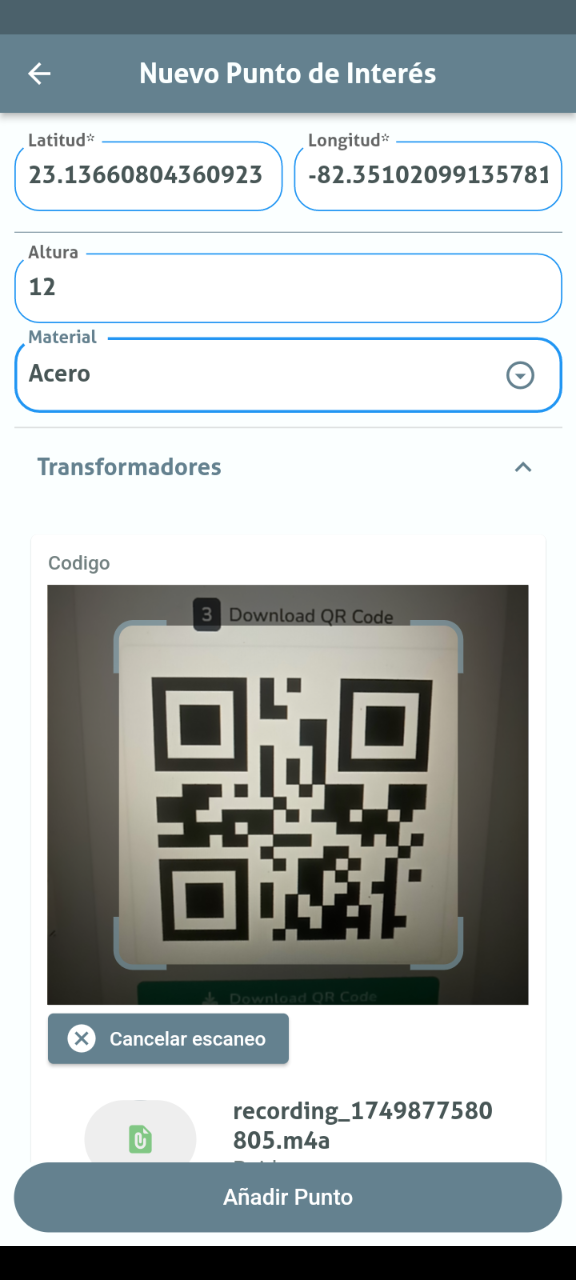
\includegraphics[width=\textwidth]{images/functionality_test/medias2.png}
    \caption{Escaneo de código QR desde la aplicación}
    \label{fig:medias1}
  \end{minipage}
  \hspace{0.02\textwidth}
  \begin{minipage}[b]{0.3\textwidth}
    \centering
    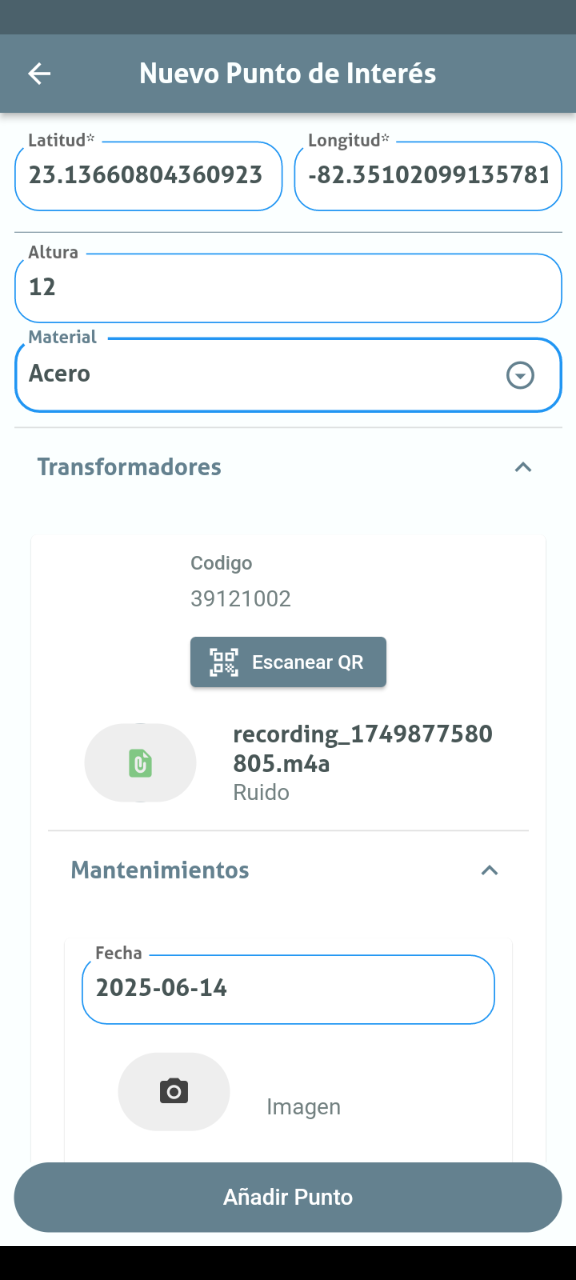
\includegraphics[width=\textwidth]{images/functionality_test/medias_1.png}
    \caption{Visualización de código QR escaneado}
    \label{fig:medias2}
  \end{minipage}
  \hspace{0.02\textwidth}
  \begin{minipage}[b]{0.3\textwidth}
    \centering
    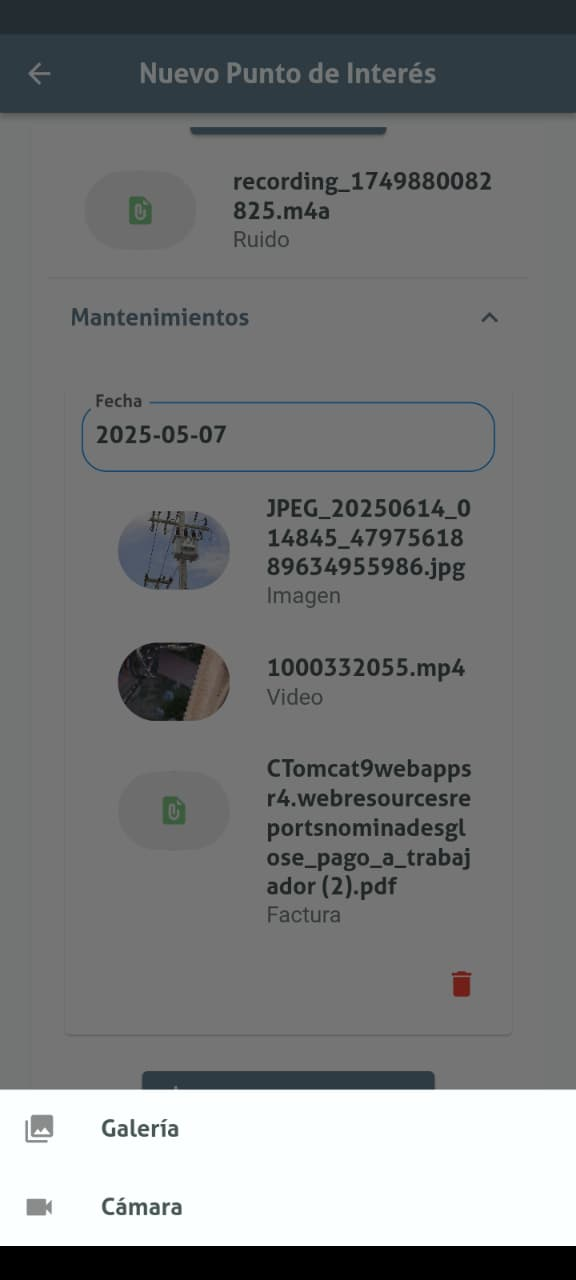
\includegraphics[width=\textwidth]{images/functionality_test/medias_3.jpg}
    \caption{Opciones para cargar un video}
    \label{fig:medias3}
  \end{minipage}
\end{figure}

\section{Prueba 4: Guardado y exportación de datos a formato Excel.}
\begin{itemize}
  \item \textit{Objetivo:} Comprobar que los datos ingresados en el formulario, incluyendo los formularios anidados y multimedia, se guardan correctamente y pueden exportarse en un archivo Excel estructurado.
  \item \textit{Entrada:} Datos completados en el formulario y comando de exportación.
  \item \textit{Salida esperada:} Archivo Excel generado con la información organizada por categorías y formularios, incluyendo referencias a archivos multimedia.
\end{itemize}

El proceso de guardado y exportación de datos se realiza desde la página para mostrar todos los puntos por categorías, tal como se muestra en las Figuras \ref{fig:geodataexporter1} y \ref{fig:geodataexporter11}, lo que facilita la gestión y revisión antes de proceder a la exportación. Al profundizar en una categoría específica, como se observa en la Figura \ref{fig:geodataexporter11}, se despliegan los datos detallados correspondientes, incluyendo los formularios anidados y los elementos multimedia asociados. 

La Figura \ref{fig:geodataexporter2} evidencia la confirmación de una exportación exitosa, donde el sistema genera una carpeta con un archivo Excel estructurado que contiene toda la información organizada por categorías y formularios, junto a otra carpeta donde guarda todos los archivos multimedia relacionados con los puntos. Este archivo permite la consulta y análisis externo de los datos capturados. Complementariamente, la Figura \ref{fig:excel} muestra cómo los archivos multimedia, como videos, imágenes, etc, se vinculan dentro del proceso, asegurando que estos recursos estén disponibles y referenciados adecuadamente en el archivo exportado.

Por último, la Figura \ref{fig:foldermedias} muestra todos los archivos multimedia exportados en el directorio \textit{Medias}, evidenciando la correcta organización y almacenamiento de videos, imágenes y otros recursos asociados.

\begin{figure}[H]
  \centering
  \begin{minipage}[b]{0.3\textwidth}
    \centering
    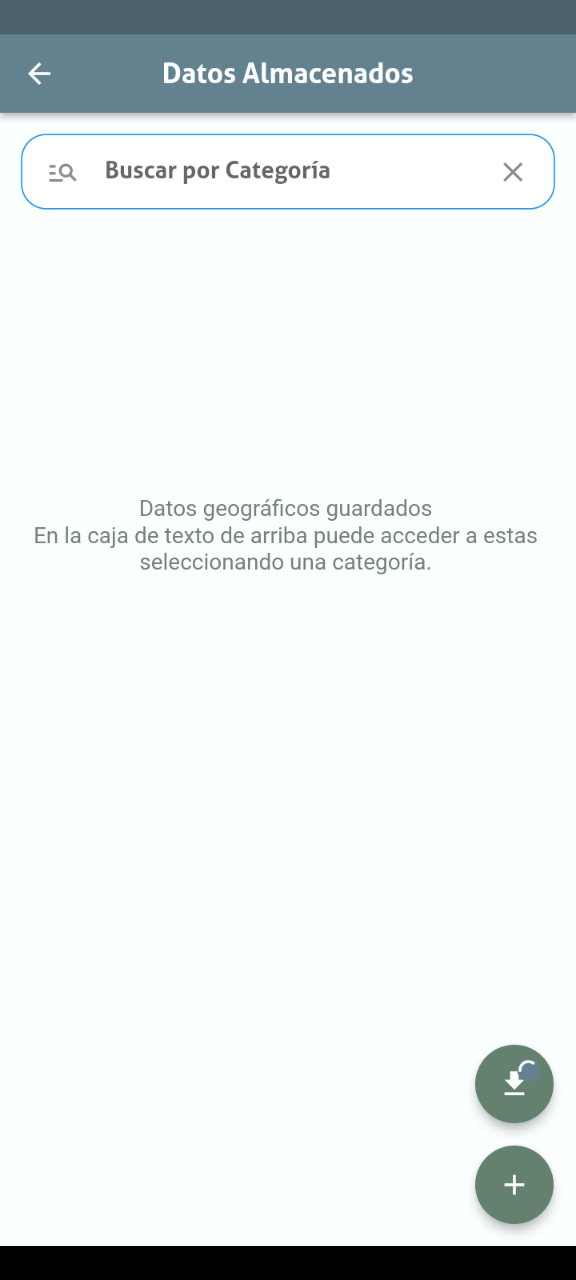
\includegraphics[width=\textwidth]{images/functionality_test/geodata_exporter1.png}
    \caption{Página de los datos por categorías}
    \label{fig:geodataexporter1}
  \end{minipage}
  \hspace{0.02\textwidth}
  \begin{minipage}[b]{0.3\textwidth}
    \centering
    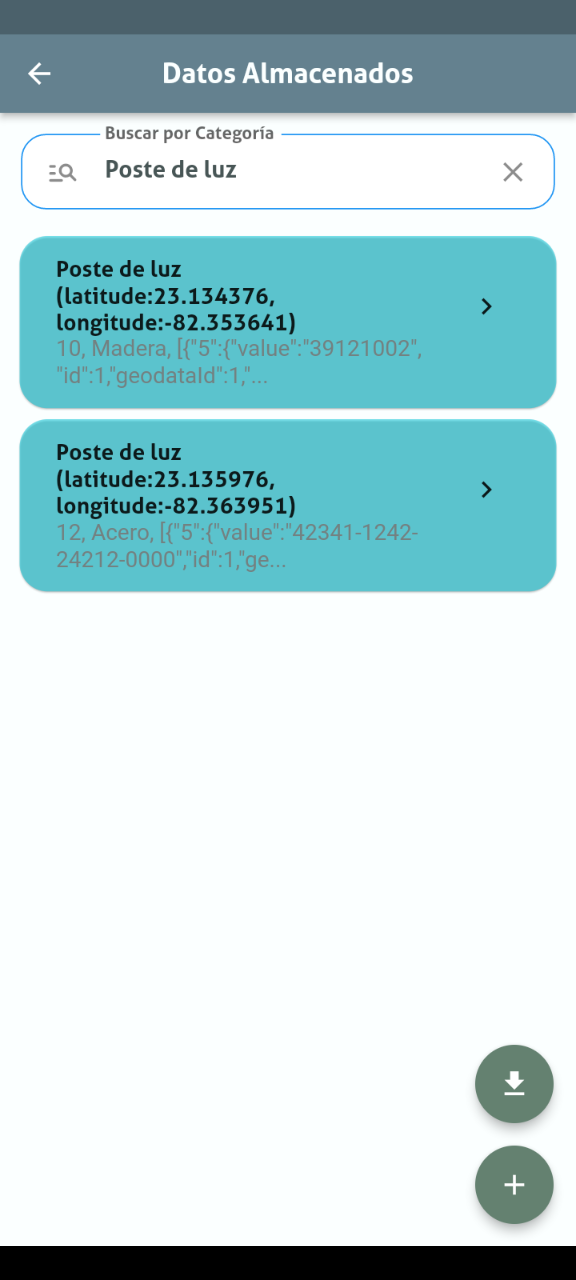
\includegraphics[width=\textwidth]{images/functionality_test/geodata_exporter11.png}
    \caption{Página de los datos de la categoría \textit{Poste de luz}}
    \label{fig:geodataexporter11}
  \end{minipage}
  \hspace{0.02\textwidth}
  \begin{minipage}[b]{0.3\textwidth}
    \centering
    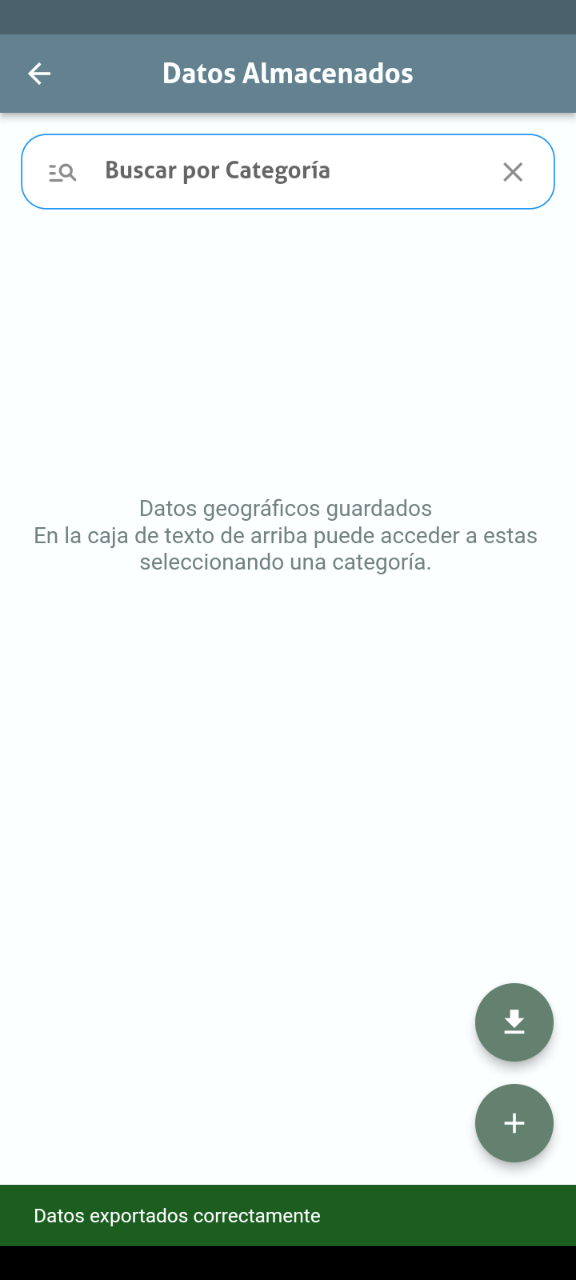
\includegraphics[width=\textwidth]{images/functionality_test/geodata_exporter2.png}
    \caption{Exportación realizada con éxito}
    \label{fig:geodataexporter2}
  \end{minipage}
\end{figure}

\begin{figure}[H]
  \centering
  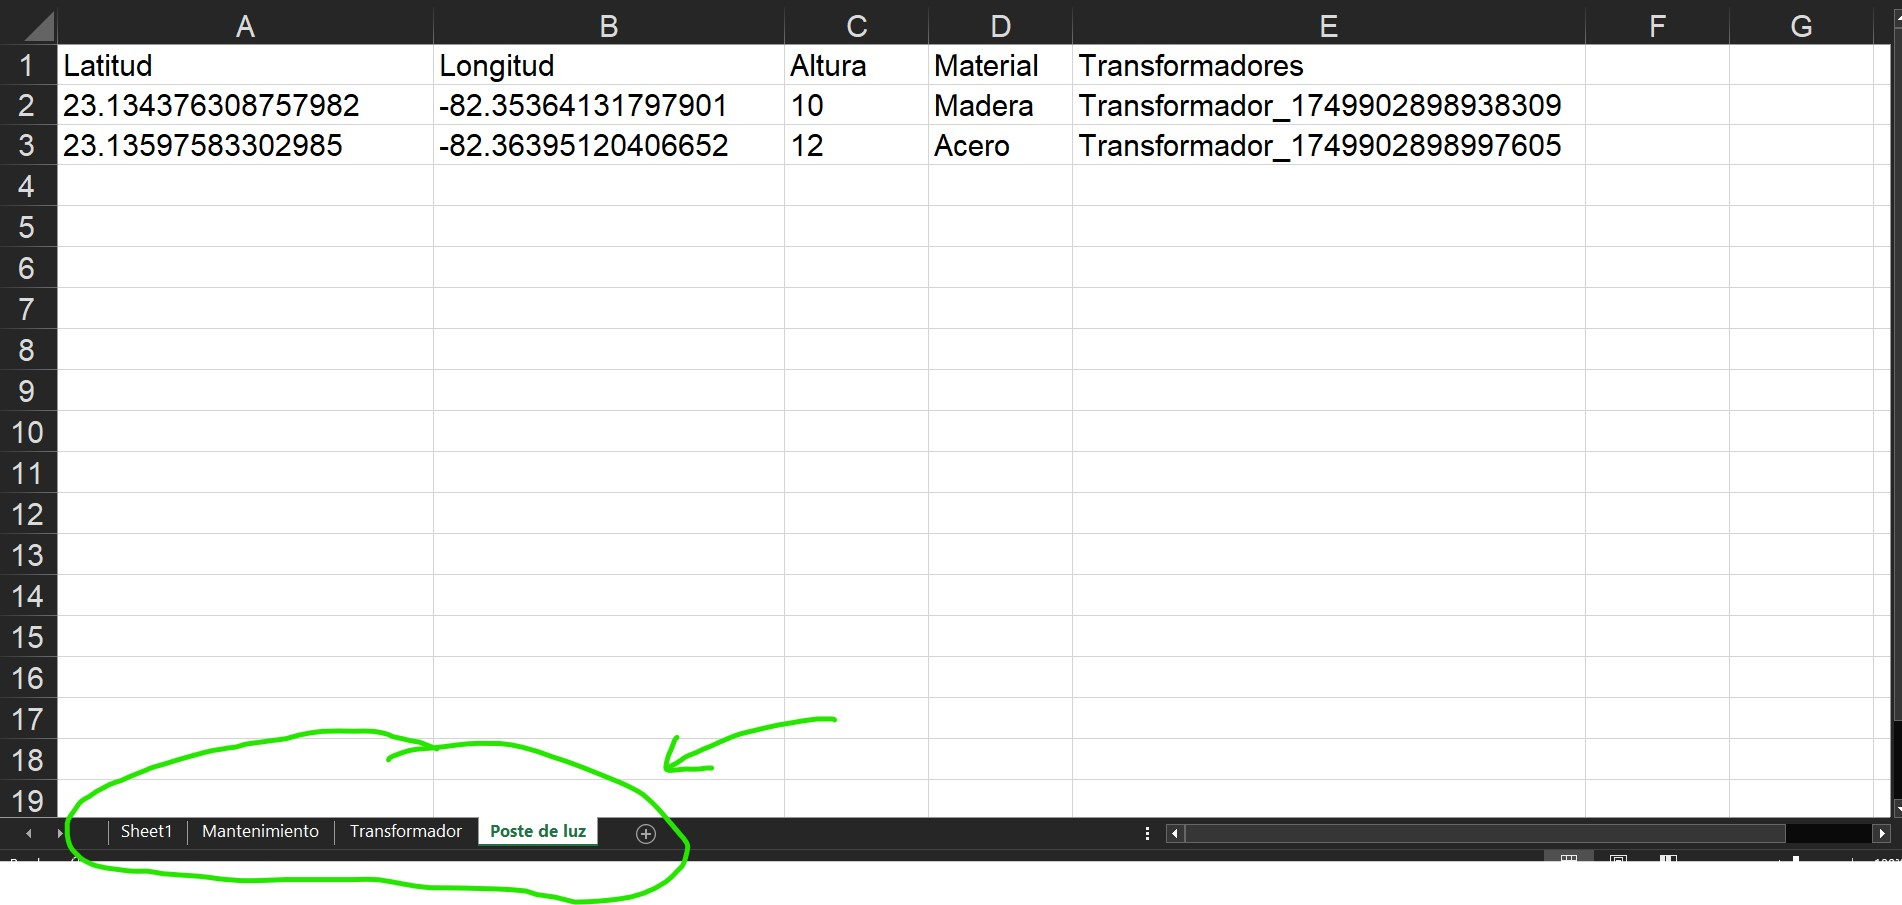
\includegraphics[width=0.7\textwidth]{images/functionality_test/excel.jpg}
  \caption{Opciones para cargar un video}
  \label{fig:excel}
\end{figure}

\begin{figure}[H]
  \centering
  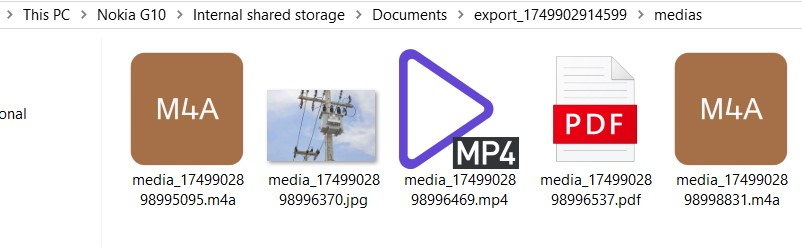
\includegraphics[width=0.7\textwidth]{images/functionality_test/folder_medias.jpg}
  \caption{Archivos multimedia del punto exportados en el directorio.}
  \label{fig:foldermedias}
\end{figure}

Estas pruebas permiten evidenciar la efectividad de la solución propuesta para abordar las necesidades reales de la empresa eléctrica en zonas rurales, demostrando la capacidad de GeoBase para manejar datos complejos, multimedia y georreferenciados, facilitando así la toma de decisiones y la optimización de recursos en el mantenimiento de la infraestructura eléctrica.

\chapter{Conclusiones y recomendaciones}

El desarrollo de la aplicación para la captura y gestión de datos georreferenciados con formularios anidados y soporte multimedia ha demostrado ser una solución efectiva y robusta para la recolección de información en campo. A través de las distintas pruebas realizadas, se ha validado que la plataforma cumple con los objetivos planteados, ofreciendo una experiencia intuitiva y funcional para los usuarios.

En primer lugar, la correcta implementación del renderizado dinámico de formularios anidados permitió que los usuarios puedan capturar datos complejos y estructurados de manera ordenada, facilitando la gestión de información relacionada a puntos georreferenciados. La capacidad de expandir y contraer subformularios garantiza una navegación eficiente sin saturar la interfaz, lo que se traduce en una mejora significativa en la usabilidad.

Asimismo, la integración de columnas especializadas para la captura de datos multimedia, como fotos, videos, notas de voz y códigos QR, amplió las posibilidades de documentación en terreno, permitiendo que la información recolectada sea más rica y completa. La correcta visualización y almacenamiento de estos datos multimedia confirma la solidez técnica del sistema para manejar diferentes tipos de contenido.

Finalmente, la funcionalidad de guardado y exportación a formato Excel estructurado asegura que toda la información capturada, incluyendo formularios anidados y referencias a archivos multimedia, pueda ser almacenada y analizada posteriormente de manera eficiente. Esta característica es crucial para la integración de la aplicación en procesos administrativos y de análisis de datos, facilitando la toma de decisiones basada en información precisa y organizada.

En conjunto, la aplicación desarrollada representa una herramienta integral para la captura de datos georreferenciados, que combina flexibilidad, usabilidad y robustez técnica, contribuyendo significativamente a la mejora de los procesos de recolección y gestión de información en campo.

Con base en los resultados obtenidos durante el desarrollo y las pruebas de la aplicación, así como en la experiencia adquirida a lo largo del proyecto, se plantean a continuación una serie de recomendaciones orientadas a mejorar y ampliar las funcionalidades del sistema. 

\begin{itemize}
  \item Implementar técnicas de optimización que reduzcan el consumo de recursos durante la captura de datos multimedia y el manejo de formularios anidados, especialmente para formularios grandes en dispositivos con capacidades limitadas.
  \item Incorporar la sincronización automática y en tiempo real con servidores remotos permitiría que los datos capturados se respalden y compartan de forma inmediata, facilitando la colaboración y evitando pérdidas de información.
  \item Continuar perfeccionando la interfaz para que la navegación entre formularios y subformularios sea aún más intuitiva, incluyendo opciones de búsqueda, filtrado y agrupación que agilicen el acceso a datos específicos.
  \item Implementar reglas de validación dinámicas y mecanismos automáticos de verificación que alerten sobre posibles errores o inconsistencias durante la entrada de datos.
  \item Desarrollar materiales de capacitación y guías de uso detalladas que faciliten la adopción de la aplicación por parte de los usuarios, asegurando un manejo adecuado y eficiente de todas las funcionalidades.
  \item Hacer extensible la exportación de los datos a otros formatos (como CSV, JSON o bases de datos), lo cual permitiría una mayor compatibilidad con diferentes herramientas y sistemas
\end{itemize}

\begin{thebibliography}{9}

  \bibitem{garcia2024}
  L. A. García López, \textit{``Geobase: aplicación móvil diseñada para el levantamiento en campo''}, \textit{Tesis de Licenciatura, Universidad de la Habana}.

  \bibitem{sarria2020} 
  F. Sarría, \textit{``Sistemas de Información Geográfica''}, 2020. [Online]. Disponible: \url{https://www.um.es/geograf/sigmur/sigpdf/temario_in.pdf}
  
  \bibitem{castro2018}
  S. Castro, \textit{``Aplicaciones móviles para la recogida y notificación de datos en campo sobre las propiedades de Managua, Nicaragua''}, \textit{Tesis de Licenciatura, Universidad de la Habana}
  
  \bibitem{rivero2019} 
  A. Rivero, \textit{``NTCollector: aplicación móvil para manejo de redes geográficas con formularios dinámicos''}, \textit{Tesis de Licenciatura, Universidad de la Habana}.

  \bibitem{ceri1984}
  S. Ceri, G. Gottlob, y L. Tanca, \textit{``A Comparative Study of Various Nested Normal Forms''}, \textit{IEEE Transactions on Software Engineering}, vol. SE-10, no. 5, pp. 569--579, 1984. [Online]. Disponible: \url{https://doi.org/10.1109/TSE.1984.5010245}

  \bibitem{esriFieldMaps}
  Esri, \textit{``Introducción a ArcGIS Field Maps''}, 2024. [En línea]. Disponible: \url{https://doc.arcgis.com/es/field-maps/get-started/get-started.htm}

  \bibitem{merginmapsdocs}
  Mergin Maps, \textit{``Mergin Maps Documentation''}, 2024. [En línea]. Disponible: \url{https://merginmaps.com/docs/}

  \bibitem{giscloudhow}
  GIS Cloud, \textit{``How it works''}, 2024. [En línea]. Disponible: \url{https://www.giscloud.com/how-it-works/}

  \bibitem{qgisdocs}
  QGIS Development Team, \textit{QGIS 3.40 Documentation} 2024. [En línea]. Disponible: \url{https://docs.qgis.org/3.40/en/docs/index.html}

  \bibitem{martin2017}
  R. C. Martin, \textit{``Clean Architecture: A Craftsman's Guide to Software Structure and Design''}, Prentice Hall, 2017.

  \bibitem{record2024}
  Dart Packages, \textit{``record: A package for recording and playing back audio''}, 2024. [Online]. Disponible: \url{https://pub.dev/packages/record}

  \bibitem{excel2024}
  Dart Packages, \textit{``excel: A library for creating, reading, and updating Excel (XLSX) files in Dart/Flutter''}, 2024. [Online]. Disponible: \url{https://pub.dev/packages/excel}
  
  \bibitem{qrcodescanner2024}
  Dart Packages, \textit{``qr\_code\_scanner: A Flutter plugin for scanning QR codes using the device's camera''}, 2024. [Online]. Disponible: \url{https://pub.dev/packages/qr_code_scanner}

  \bibitem{path2024}
  Dart Team, \textit{``path: A comprehensive library for path manipulation in Dart''}, 2024. [Online]. Disponible: \url{https://pub.dev/packages/path}

\end{thebibliography}

\end{document}
